%%
%% Automatically generated file from Doconce source
%% (https://github.com/hplgit/doconce/)
%%
% #ifdef PTEX2TEX_EXPLANATION
%%
%% The file follows the ptex2tex extended LaTeX format, see
%% ptex2tex: http://code.google.com/p/ptex2tex/
%%
%% Run
%%      ptex2tex myfile
%% or
%%      doconce ptex2tex myfile
%%
%% to turn myfile.p.tex into an ordinary LaTeX file myfile.tex.
%% (The ptex2tex program: http://code.google.com/p/ptex2tex)
%% Many preprocess options can be added to ptex2tex or doconce ptex2tex
%%
%%      ptex2tex -DMINTED myfile
%%      doconce ptex2tex myfile envir=minted
%%
%% ptex2tex will typeset code environments according to a global or local
%% .ptex2tex.cfg configure file. doconce ptex2tex will typeset code
%% according to options on the command line (just type doconce ptex2tex to
%% see examples). If doconce ptex2tex has envir=minted, it enables the
%% minted style without needing -DMINTED.
% #endif

% #define PREAMBLE

% #ifdef PREAMBLE
%-------------------- begin preamble ----------------------

\documentclass[%
twoside,                 % oneside: electronic viewing, twoside: printing
final,                   % or draft (marks overfull hboxes, figures with paths)
10pt]{article}

\listfiles               % print all files needed to compile this document

\usepackage{relsize,epsfig,makeidx,color,setspace,amsmath,amsfonts}
\usepackage[table]{xcolor}
\usepackage{bm,microtype}

\usepackage{ptex2tex}

% #ifdef MINTED
\usepackage{minted}
\usemintedstyle{default}
% #endif

\usepackage[T1]{fontenc}
%\usepackage[latin1]{inputenc}
\usepackage[utf8]{inputenc}

\usepackage{lmodern}         % Latin Modern fonts derived from Computer Modern

% Hyperlinks in PDF:
\definecolor{linkcolor}{rgb}{0,0,0.4}
\usepackage[%
    colorlinks=true,
    linkcolor=linkcolor,
    urlcolor=linkcolor,
    citecolor=black,
    filecolor=black,
    %filecolor=blue,
    pdfmenubar=true,
    pdftoolbar=true,
    bookmarksdepth=3   % Uncomment (and tweak) for PDF bookmarks with more levels than the TOC
            ]{hyperref}
%\hyperbaseurl{}   % hyperlinks are relative to this root

\setcounter{tocdepth}{2}  % number chapter, section, subsection

% Tricks for having figures close to where they are defined:
% 1. define less restrictive rules for where to put figures
\setcounter{topnumber}{2}
\setcounter{bottomnumber}{2}
\setcounter{totalnumber}{4}
\renewcommand{\topfraction}{0.85}
\renewcommand{\bottomfraction}{0.85}
\renewcommand{\textfraction}{0.15}
\renewcommand{\floatpagefraction}{0.7}
% 2. ensure all figures are flushed before next section
\usepackage[section]{placeins}
% 3. enable begin{figure}[H] (often leads to ugly pagebreaks)
%\usepackage{float}\restylefloat{figure}

% prevent orhpans and widows
\clubpenalty = 10000
\widowpenalty = 10000

% --- end of standard preamble for documents ---


% insert custom LaTeX commands...

\raggedbottom
\makeindex

%-------------------- end preamble ----------------------

\begin{document}

% #endif


% ------------------- main content ----------------------



% ----------------- title -------------------------

\thispagestyle{empty}

\begin{center}
{\LARGE\bf
\begin{spacing}{1.25}
Geographic models 
\end{spacing}
}
\end{center}

% ----------------- author(s) -------------------------

\begin{center}
{\bf Torbjørn Seland${}^{}$} \\ [0mm]
\end{center}

    \begin{center}
% List of all institutions:
\end{center}

% ----------------- end author(s) -------------------------

\begin{center}
Nov 15, 2014
\end{center}

\vspace{1cm}


\tableofcontents


\vspace{1cm} % after toc




\section{Introduction}
This chapter will introduce a new model for epidemic diseases. By expand the ODE system from previous chapter to consist of a geographic spread of epidemics. The first section \emph{Simple system for spatial spread} will build on the simple SIR model presented in previous chapter and be based on Murray \cite{murray2003mathematical}. A couple of tests will be done on the model to verify that the implementation is done correct. The parameters from \emph{Epidemic from the English School} will be used in this model and the result will be compared against the ODE system. The position of the infected student will be compared against the number of infected each day. The last section \emph{Zombiefication} will compare and develop the zombie model presented in the previous chapter.

\section{Simple system for spatial spread}
A spatial variable, \textbf{x} will now be introduced to the new model. This means that the position has an effect on the change in each class. The system that will be shown here, will be based on the simple ODE system presented in the previous chapter. The difference will be the diffusion part added to each equation. The system can be seen in eq(\ref{eq:simple_PDE}). 
\begin{equation} \label{eq:simple_PDE}
	\begin{aligned}
	\frac{\partial S}{\partial t} &= -rIS + D\nabla ^2 S\\
	\frac{\partial I}{\partial t} &= rIS- aI + D\nabla ^2 I\\
	\frac{\partial R}{\partial t} &= aI + D\nabla ^2 R
	\end{aligned}
\end{equation}
All three classes have the same diffusion coefficient, $D$. This give the three groups the same diffusion speed. Often will this differ between groups and will be study later in \emph{Zombiefication}.The two parts $rIS$ and $aI$ will work in the same way as in the ODE system. Since this model taking the position into account, the idea is to model a group of infective that moves into a uniform population with susceptible, which is spread around with the density $S_0$. Then the geotemporal spread can be seen. The problem will first be consider as one-dimensional. The system can be nondimensionalise by writing 
\begin{equation} \label{eq:constants_nondimensional}
	\begin{aligned}
	I^* =\frac{I}{S_0},&\quad I^* = \frac{I}{S_0},&\quad R^*= \frac{R}{S_0},&\\
	x^* =\left(\frac{rS_0}{D}\right)^{1/2}x,&\quad t^*=rS_0t,&\quad \lambda =\frac{a}{rS_0},&
	\end{aligned}
\end{equation}
$S_0$ is used as a representative population. Now the model(\ref{eq:simple_PDE}) can be expressed as in eq(\ref{eq:simple_non_PDE}). The asterisks have been dropped to make it easier to read.
\begin{equation} \label{eq:simple_non_PDE}
	\begin{aligned}
	\frac{\partial S}{\partial t} &= -IS + \frac{\partial^2 S}{\partial x^2},\\
	\frac{\partial I}{\partial t} &= IS- \lambda I + \frac{\partial^2 I}{\partial x^2},\\
	\frac{\partial R}{\partial t} &= \lambda I + \frac{\partial^2 R}{\partial x^2},
	\end{aligned}
\end{equation}
The three parameters $r$, $a$ and $D$ have now been replaced by $\lambda$. The \emph{reproduction rate} that was presented for the ODE model can be seen by $1/\lambda $. This has a couple of equivalent meanings. $1/\lambda$ can be seen as the number of secondary infections produced by one primary infected. It can also be used to measure two different time scales. The first one, $1/(rS_0)$, measure the contagious time of the disease. The second one can look at the life expectancy for an infective. This can be described $1/a$. 
\subsection{Travelling wave 1D}
The problem that this section will focus on, is the travelling wave. The travelling wave describe how a disease travel through geographic area of humans. This will be shown here by sending a pulse of infected into a group of susceptible. A travelling wave solution will be described as follows,
\begin{equation}
I(x,t)=I(z),\quad S(x,t)=S(z),\quad R(x,t) = R(z),\quad z = x-ct,
\end{equation}
Here the value $c$ will be the wave speed. This represents a wave of constant shape that travels in the positive x-direction. These can now be inserted into (\ref{eq:simple_non_PDE}). This gives the ordinary system(\ref{eq:ord_diff_sys})
\begin{equation} \label{eq:ord_diff_sys}
	\begin{aligned}
	S'' + cS' - IS &= 0,\\
	I'' + cI' + I(S-\lambda)&=0\\
	R'' + cR  + I\lambda &=0
	\end{aligned}
\end{equation}
This gives an eigenvalue problem to find the range of $\lambda$ so that $c$ always will be positive. The values of $S$, $I$ and $R$ also has to stay nonnegative. This leads to
\begin{equation} 
	\begin{aligned}
	0 \leq S(-\infty) < S(\infty)&=1\\
	I(-\infty)=I(\infty)&=0,\\
	1 \geq R(-\infty)\geq R(\infty) &= 0
	\end{aligned}
\end{equation}

% MOVIE:[plots/Travelling_wave.webm, height=500 width=600] This simulation is based on (\ref{eq:ord_diff_sys}) with $\lambda=0.5$. The initial data is sat to $S(x,0)=1$ and $R(x,0)=0$. The left side of the \emph{Infective} class, $I(0,0), is based on a gaussian curve. The rest is sat to be zero.


\begin{figure}[ht]
  \centerline{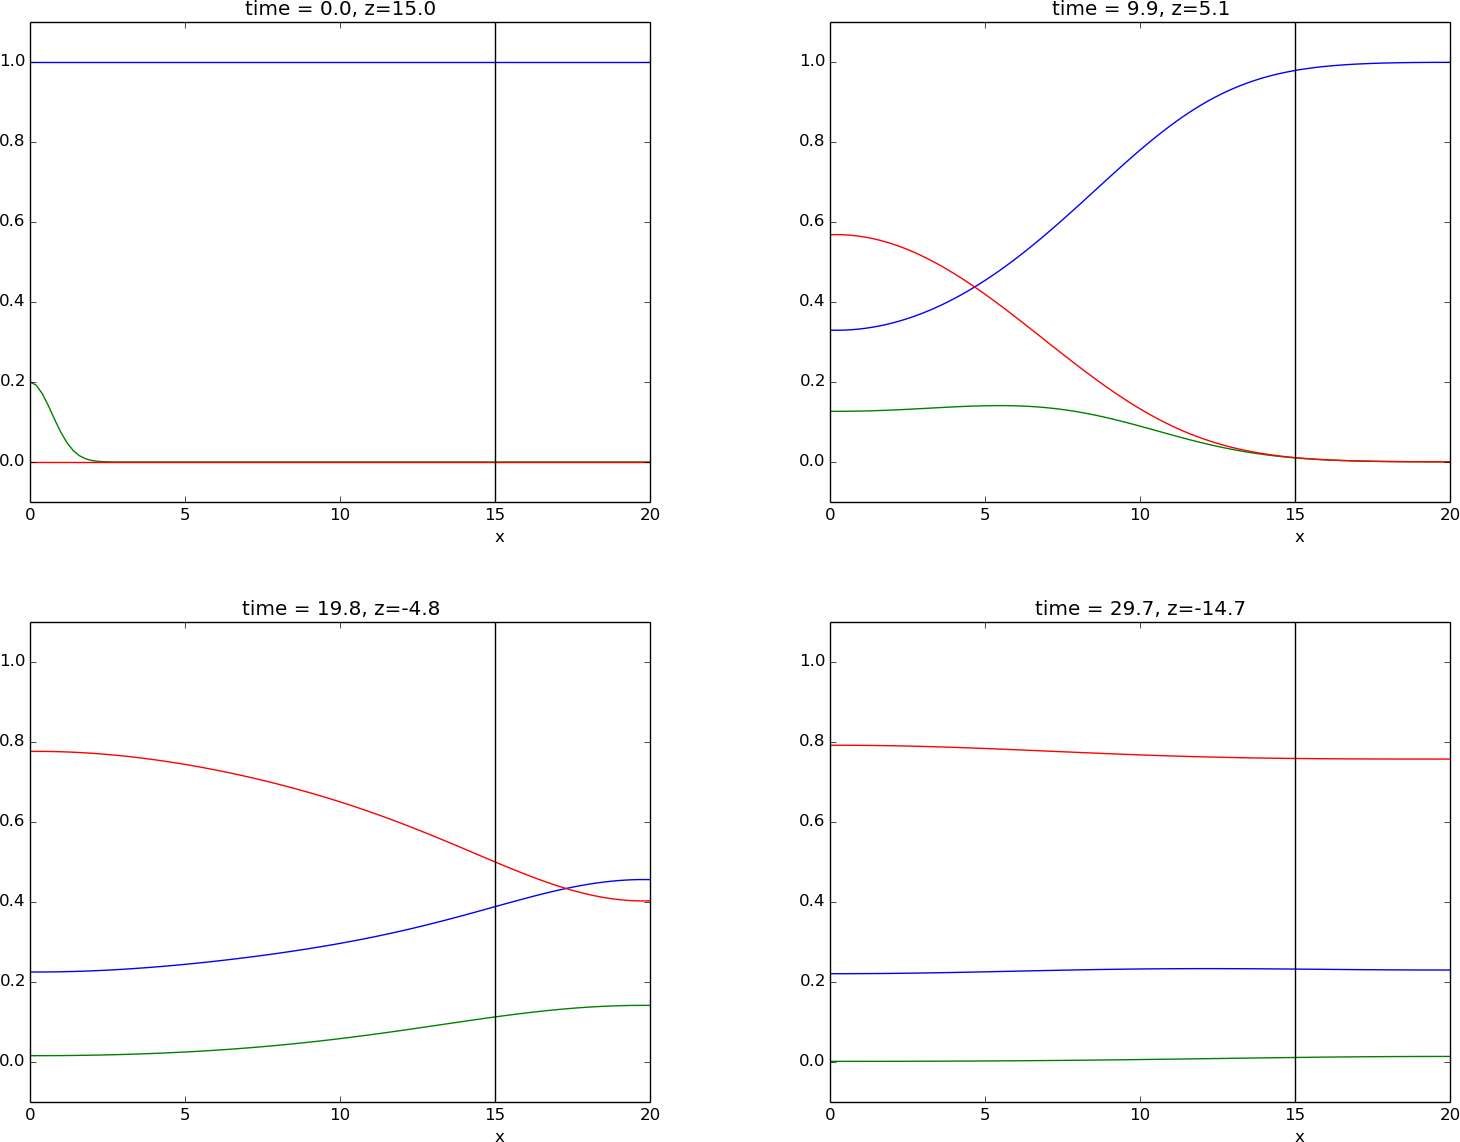
\includegraphics[width=0.8\linewidth]{plots/trav_wave_sub.eps}}
  \caption{
  \label{fig:1D_sub} A gauss curve is inserted on the left side. This causes an epidemic wave. The size is measured at $x=15$ and can be seen in figure (\ref{fig:1D_tw}).
  }
\end{figure}
%\clearpage % flush figures fig:1D_sub



\begin{figure}[ht]
  \centerline{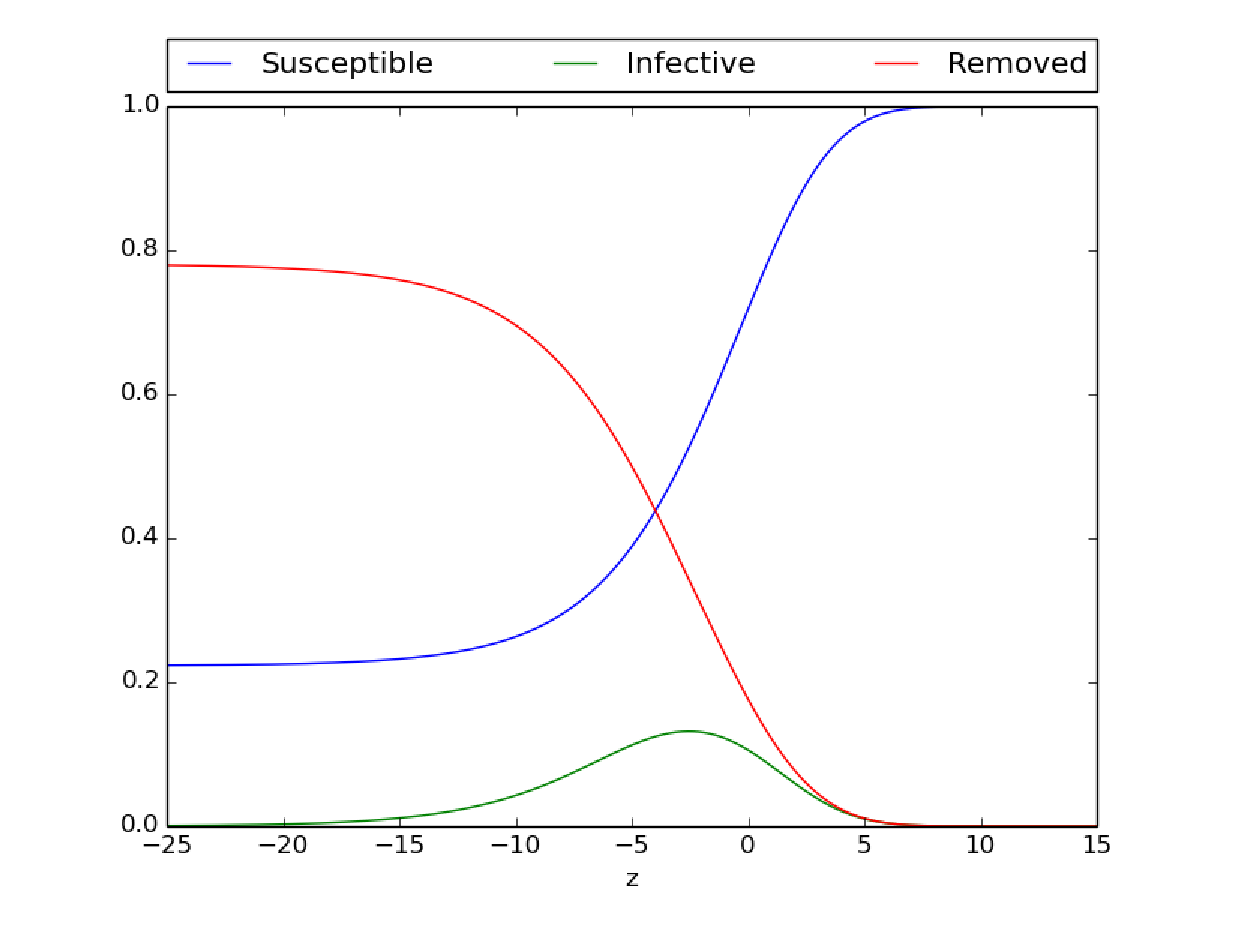
\includegraphics[width=0.9\linewidth]{plots/epidemic_wave_z_lambda_0_5.eps}}
  \caption{
  \label{fig:1D_tw} This shows the travelling wave measures at at $x=15$ in figure(\ref{fig:1D_sub})
  }
\end{figure}
%\clearpage % flush figures fig:1D_tw


The system(\ref{eq:ord_diff_sys}) is a fourth order phase space system. The lower bound time speed for $c$ can be found. J.D Murray shows this in \emph{kite{Murray}}. The \emph{Infective} class in the system(\ref{eq:ord_diff_sys}) can be linearised when $z\rightarrow \infty$ $S\rightarrow 1$ and $I \rightarrow 0$. The result then become 
\begin{equation}
	I'' + cI' + I(S-\lambda) \approx 0 
\end{equation}
This can be found by
\begin{equation}
I(z) \varpropto \exp\left[(-c \pm {c^2 -4(1-\lambda)}^{1/2})z/2\right]
\end{equation}
It is required that $I(z)\rightarrow 0$, but not under. This means that the solution cannot oscillate around 0. If a travelling wave exist, it has to satisfy
\begin{equation}
	c \geq 2(1-\lambda)^{1/2}, \lambda < 1
\end{equation}
If $\lambda > 1$, no travelling wave will exist. Then the disease will die out. The terms defined in (\ref{eq:constants_nondimensional}) will give the threshold conditions,
\begin{equation}
	\lambda = \frac{a}{rS_0} < 1
\end{equation}
This is the same value that was given for the ODE model in the previous chapter.
\subsection{Verifying the solution}
\paragraph{Constant solution.}
To verify this solution a couple of tests can be done one the system. The first test will be a constant test, where a known constant solution is given. A look at the previous system will give an idea on performing the test.
\begin{equation} \label{eq:simple_non_PDE2}
	\begin{aligned}
	\frac{\partial S}{\partial t} &= -IS + \frac{\partial^2 S}{\partial x^2},\\
	\frac{\partial I}{\partial t} &= IS- \lambda I + \frac{\partial^2 I}{\partial x^2},\\
	\frac{\partial R}{\partial t} &= \lambda I + \frac{\partial^2 R}{\partial x^2},
	\end{aligned}
\end{equation}
By setting the solutions to constants, $S = C_s,I=C_i,R=C_r$, the value of $C_i$ has to be 0. This is a poor test and several bugs can escape. The following system can be expanded by adding $\beta R$ to the system. This give the chance to check the value of $R$ and the constants can be set to a different value than 0.  
\begin{equation} \label{eq:constant_PDE}
	\begin{aligned}
	C_IC_S &= \beta C_r \\
	C_IC_S &= \lambda C_I \\
	\lambda C_I &= -\beta C_R 
	\end{aligned}
\end{equation}
The constant values can freely be chosen. Here they are sat to $C_S = 1.2,C_I=0.8,C_R=0.6$. This give $\lambda=1.2$ and $\beta=1.6$. A test can be made

\bpycod
def test_constant_solution():
    """
    Test problem where u=u_const is the exact solution, to be
    reproduced (to machine precision) by any relevant method.
    """
    def exact_solution(t):
        return C_s,C_i,C_r
    
    def lam(t,x):
        return C_s

    def beta(t,x):
        return (C_s*C_i)/float(C_r)

    #Constant values
    C_s = 1.2
    C_i = 0.8
    C_r = 0.6
    
    #lam = C_s
    #beta = (lam*C_i)/float(C_r)
    
    T = 2; Nt = 200
    X = 20; Nx = 40
    S_1 = np.ones(Nx+3)*C_s
    I_1 = np.ones(Nx+3)*C_i
    R_1 = np.ones(Nx+3)*C_r
    
    t,x,S,I,R = simple_PDE(T,Nx,Nt,X,lam,beta,S_1,I_1,R_1)
    
    S_e,I_e,R_e = exact_solution(t)
    difference = abs(S_e - S).max()  # max deviation
    tol = 1E-14
    assert difference < tol

    difference = abs(I_e - I).max()  # max deviation
    tol = 1E-14
    assert difference < tol

    difference = abs(R_e - R).max()  # max deviation
    tol = 1E-14
    assert difference < tol
\epycod

This test was fine and next test that can be done on the system is a Manufactured solution
\paragraph{Manufactured solution.}
By constructing a function to each equation in the system (\ref{eq:simple_non_PDE}), a manufactured solution can be created. Here $S$,$I$ and $R$ are pre produced. The system will be
\begin{equation} \label{eq:simple_non_PDE2}
	\begin{aligned}
	\frac{\partial S}{\partial t} &= -IS + \frac{\partial^2 S}{\partial x^2}+f(x,t),\\
	\frac{\partial I}{\partial t} &= IS- \lambda I + \frac{\partial^2 I}{\partial x^2}+g(x,t),\\
	\frac{\partial R}{\partial t} &= \lambda I + \frac{\partial^2 R}{\partial x^2}+h(x,t),
	\end{aligned}
\end{equation}
where $f$,$g$ and $h$ are constructed functions to achieve the expected results for $S$, $I$ and $R$. In this case the functions will be:
\begin{equation}
	\begin{aligned}
	f(x,t) = \frac{\partial S}{\partial t} + IS - \frac{\partial^2 S}{\partial x^2}\\
	g(x,t) = \frac{\partial I}{\partial t} - IS + \lambda I - \frac{\partial^2 I}{\partial x^2}\\
	h(x,t) = \frac{\partial R}{\partial t} -\lambda I - \frac{\partial^2 R}{\partial x^2},
	\end{aligned}
\end{equation}
When choosing the expected function for the classes, it is important that the fulfill the boundary conditions
\begin{equation}
    u_x(0,t) = u_x(X,t) = 0
\end{equation}
The quantities have here been sat to:
\begin{equation}
	\begin{aligned}
    S(x,t) = cos(\frac{\pi}{X}x)t\\
    I(x,t) = cos(\frac{\pi}{X}x)t\\
    R(x,t) = cos(\frac{\pi}{X}x)t
	\end{aligned}
\end{equation}
Now \code{sympy} can be used to do the calculations

\bpycod
>>> from sympy import *
>>> x,t,lam = symbols('x t lam')
>>> def s_simple(x,t):
...     return cos(pi*x)*t
... 
>>> def i_simple(x,t):
...     return cos(pi*x)*t
... 
>>> def r_simple(x,t):
...     return cos(pi*x)*t
... 
>>> for x_point in 0,1:
...     print "s_x(%s,t): ", % x_point,
>>> for x_point in 0,1:
...     print "s_x(%s,t): " % x_point,
...     print diff(s_simple(x,t),x).subs(x,x_point).simplify()
...     print "i_x(%s,t): " % x_point,
...     print diff(i_simple(x,t),x).subs(x,x_point).simplify()
...     print "r_x(%s,t): " % x_point,
...     print diff(r_simple(x,t),x).subs(x,x_point).simplify()
... 
s_x(0,t):  0
i_x(0,t):  0
r_x(0,t):  0
s_x(1,t):  0
i_x(1,t):  0
r_x(1,t):  0
>>> s = s_simple(x,t)
>>> i = i_simple(x,t)
>>> r = r_simple(x,t)
>>> f = diff(s,t)+i*s-diff(diff(s,x),x)
>>> print f.simplify()
(t**2*cos(pi*x) + pi**2*t + 1)*cos(pi*x)
>>> g = diff(i,t)-i*s+lam*i-diff(diff(i,x),x)
>>> print g.simplify()
(lam*t - t**2*cos(pi*x) + pi**2*t + 1)*cos(pi*x)
>>> h = diff(r,t)-lam*i-diff(diff(r,x),x)
>>> print h.simplify()
(-lam*t + pi**2*t + 1)*cos(pi*x)
\epycod
Which give
\begin{equation}
	\begin{aligned}
	f(x,t) &= (t^2\cos(\pi x) + \pi^2t + 1)\cos(\pi x)\\
	g(x,t) &= (\lambda t - t^2\cos(\pi x) + \pi^2t + 1)\cos(\pi x)\\
	h(x,t) &= (-\lambda t + \pi^2t + 1)\cos(\pi x)
	\end{aligned}
\end{equation}

The following manufactured test will then be
\bpycod
def test_manufactured_solution(T,Nt,X,Nx):
    """
    Test problem where u=c*t+I is the exact solution, to be
    reproduced (to machine precision) by any relevant method.
    """
    
    def exact_solution_S(t,x):
        return np.cos(np.pi*x)*t

    def exact_solution_I(t,x):
        return np.cos(np.pi*x)*t

    def exact_solution_R(t,x):
        return np.cos(np.pi*x)*t


    def beta(t,x):
        return exact_solution_S(t,x)*exact_solution_I(t,x)/exact_solution_R(t,x)
    lam = 1
    def f(t,x):
        return (t**2*np.cos(np.pi*x) + np.pi**2*t + 1)*np.cos(np.pi*x) 

    def g(t,x):
        return (lam*t - t**2*np.cos(np.pi*x) + np.pi**2*t + 1)*np.cos(np.pi*x)

    def h(t,x):
        return (-lam*t + np.pi**2*t + 1)*np.cos(np.pi*x)
        

    dx = X/float(Nx)
    dt = T/float(Nt)
    S_1 = exact_solution_S(0,np.linspace(0-dx,X+dx,Nx+3))
    I_1 = exact_solution_I(0,np.linspace(0-dx,X+dx,Nx+3))
    R_1 = exact_solution_R(0,np.linspace(0-dx,X+dx,Nx+3))
     
    t,x,S,I,R = simple_PDE(T,Nx,Nt,X,lam,beta,S_1,I_1,R_1,f,g,h)
    S_e = exact_solution_S(t[-1],x)
    I_e = exact_solution_I(t[-1],x)
    R_e = exact_solution_R(t[-1],x)
    
    difference_S = abs(S_e - S).max()  # max deviation

    
    #for i in range(4):
    #    print "n",i,"S_e",exact_solution_S(t[i],x)
    
    #print "S",S
    #t_tot = np.sum(t[:-1])
    #print "t_tot",t_tot
    #difference_exp = t_tot*dt*np.cos(x*np.pi)*((2*(np.cos(np.pi*dx)-1))/dx**2+np.pi**2)
    #print "diff_exp", (abs(difference_exp)).max()
    print "diff",difference_S
    #tol = 1E-14
    #assert difference < tol
    
    difference_I = abs(I_e - I).max()  # max deviation
    #print "diff",difference_I
    #tol = 1E-14
    #assert difference < tol
   
    difference_R = abs(R_e - R).max()  # max deviation
    #print "diff",difference_R
    #tol = 1E-14
    #assert difference < tol
    return difference_S,difference_I,difference_R
\epycod

\paragraph{Convergence rate.}
The program can be controlled by checking the convergence rate. The error term can be described as  
\begin{equation} \label{eq:error}
    \epsilon = C_x\Delta x^2 + C_t \Delta t
\end{equation}
With equation(\ref{eq:error}, the expected convergence rate can be found for both $\Delta x$ and $\Delta t$. To be able to separate the $\Delta$'s, the other value has to be close to eliminated. If the value for $\Delta x$ wants to be found,  $\Delta t \ll \Delta x$ has to be fullfilled. This will lead to $C_t\Delta t \approx 0$, and the error term for $\Delta x$ can be found. The opposite thing can  be done for $\Delta t$. A table for the error is produced for different values for $\Delta t = 0.05$ and $\Delta x=0.1$.


\begin{quote}
\begin{tabular}{ccccc}
\hline
\multicolumn{1}{c}{  } & \multicolumn{1}{c}{ dx } & \multicolumn{1}{c}{ dx/2 } & \multicolumn{1}{c}{ dx/4 } & \multicolumn{1}{c}{ dx/8 } \\
\hline
dt     & 9.8E-3 & -      & -      & -      \\
dt/4   & 9.9E-3 & 2.5E-3 & -      & -      \\
dt/8   & 9.9E-3 & 2.5E-3 & 6.1E-4 & -      \\
dt/16  & 9.9E-3 & 2.5E-3 & 6.1E-4 & 1.5E-4 \\
\hline
\end{tabular}
\end{quote}

\noindent
% 0.00988006143376,0.00246039081619,-,-
% 0.00988361769746,0.00246127510994,0.000614719954035
% 0.00988450717896,0.00246149628689,0.000614775174047,0.000153656409034

\paragraph{The spatial error.}
The table above gives an insight on how the error develops when reducing $\Delta t$ and $\Delta x$. By studying the row where $\Delta t/16$, the $C_t \Delta t$ can be seen as close to negligible in equation(\ref{eq:error}. The error can then be expressed 
\begin{equation}
    \epsilon \propto \Delta x^r
\end{equation}
The value is expected to be $r=2$, since Crank Nicolson is used in the spatial discretization. This gives a 2.order error. By comparing the error for different $\Delta x$, the convergence rate, $r$, can be expressed, 
\begin{equation} \label{eq:conv_rate}
 r_{12} \simeq \frac{\log(\epsilon_1/\epsilon_2)}{\log(\Delta x_1/\Delta x_2)}
\end{equation}
Since the table above has four different error values, these can be used to give three different convergence rates. $\Delta x_1 = dx, \Delta x_2 = dx/2...$. The same labeling will be done for the different error values, $\epsilon$.

\begin{quote}
\begin{tabular}{cccc}
\hline
\multicolumn{1}{c}{  } & \multicolumn{1}{c}{ $\epsilon_1/\epsilon_2$ } & \multicolumn{1}{c}{ $\epsilon_2/\epsilon_3$ } & \multicolumn{1}{c}{ $\epsilon_3/\epsilon_4$ } \\
\hline
r                       & 2.0056                  & 2.0014                  & 2.0004                  \\
\hline
\end{tabular}
\end{quote}

\noindent
Here the rate goes towards 2, and a 2.order convergence rate seems to be fulfilled.
\paragraph{The temporal error.}
The temporal error is quite hard to find because the \emph{Stability criteria} which is about
\begin{equation} \label{eq:stability_cr}
 2\Delta t \leq \Delta x^2
\end{equation}
This results in the case that $\Delta x \ll \Delta t$ is impossible, because this only leads to an unstable solution. By looking at the column for $\frac{\Delta x}{8}$, the only stable solution is for ${\Delta t}{16}$. Therefore the technique used for the spatial error cannot be used here. By studying the diagonal numbers in the table, the expected convergence rate is fulfilled for both $\Delta x$, which gives $r = 2$ and for $\Delta t$ that gives $r=1$   

\subsection{Travelling wave in 2D}
The model can be discretized for a 2D simulation since an epidemic disease will spread geographically. The non dimensional system (\ref{eq:simple_non_PDE}) used in the 1D simulation above can be discretized with Forward Euler in time and Crank Nicolson in space
\begin{equation} \label{eq:SIR_disc}
	\begin{aligned}
    \frac{S^{n+1}_{i,j}-S^n_{i,j}}{\Delta t} &= -I^{n}_{i,j}S^{n}_{i,j} + \left(\frac{S^{n}_{i-1,j}-2S^{n}_{i,j}+S^{n}_{i+1,j}}{\Delta x^2}+\frac{S^{n}_{i,j-1}-2S^{n}_{i,j}+S^{n}_{i,j+1}}{\Delta y^2}\right) \\
    \frac{I^{n+1}_{i,j}-I^n_{i,j}}{\Delta t} &= I^{n}_{i,j}S^{n}_{i,j} -\lambda I^{n}_{i,j} + \left(\frac{I^{n}_{i-1,j}-2I^{n}_{i,j}+I^{n}_{i+1,j}}{\Delta x^2}+\frac{I^{n}_{i,j-1}-2I^{n}_{i,j}+I^{n}_{i,j+1}}{\Delta y^2}\right) \\
    \frac{R^{n+1}_{i,j}-R^n_{i,j}}{\Delta t} &= \lambda I^{n}_{i,j}+\left(\frac{R^{n}_{i-1,j}-2R^{n}_{i,j}+R^{n}_{i+1,j}}{\Delta x^2}+\frac{R^{n}_{i,j-1}-2R^{n}_{i,j}+R^{n}_{i,j+1}}{\Delta y^2}\right) 
	\end{aligned}
\end{equation}
Now the known values can be placed on the right side. The system will then be
\begin{equation}
	\begin{aligned}
    S^{n+1}_{i,j} &= S^{n}_{i,j}+\Delta t\left(-I^{n}_{i,j}S^{n}_{i,j} + \left(\frac{S^{n}_{i-1,j}-2S^{n}_{i,j}+S^{n}_{i+1,j}}{\Delta x^2}+\frac{S^{n}_{i,j-1}-2S^{n}_{i,j}+S^{n}_{i,j+1}}{\Delta y^2}\right)\right) \\
    I^{n+1}_{i,j} &= I^{n}_{i,j}+\Delta t\left(I^{n}_{i,j}S^{n}_{i,j} -\lambda I^{n}_{i,j} + \left(\frac{I^{n}_{i-1,j}-2I^{n}_{i,j}+I^{n}_{i+1,j}}{\Delta x^2}+\frac{I^{n}_{i,j-1}-2I^{n}_{i,j}+I^{n}_{i,j+1}}{\Delta y^2}\right)\right) \\
    R^{n+1}_{i,j} &= R^{n}_{i,j}+\Delta t\left(\lambda I^{n}_{i,j}+\left(\frac{R^{n}_{i-1,j}-2R^{n}_{i,j}+R^{n}_{i+1,j}}{\Delta x^2}+\frac{R^{n}_{i,j-1}-2R^{n}_{i,j}+R^{n}_{i,j+1}}{\Delta y^2}\right)\right) 
	\end{aligned}
\end{equation}
This results in an explicit system, which is easy to code. It consist of known values on the right side and only one unknown on the left side.
\paragraph{A gaussian wave.}
In the PDE system for the 1D equation, a Gaussian quantity of infected humans was placed on the left side in the initial value. This resulted in a wave of infected spread along the x-axis. A similar thing can be done for the 2D simulation. A couple of simulations have been done for the 2D system. The first simulation is run for a Gaussian function along $x=0$ and the second simulation is run for a Gaussian function from $x=0,y=0$ for the infected humans as initial value. Both simulations can be seen in the Appendix.  

By studying the travelling wave at a certain point, the size of the epidemic wave can be measured and compared. In these two 2D simulations, the wave will be measured in the point (15,15) while the travelling wave in the 1D simulation was measured in point(15). The two travelling waves can be seen in the figure(\ref{fig:2D_trav_wave}).


\begin{figure}[ht]
  \centerline{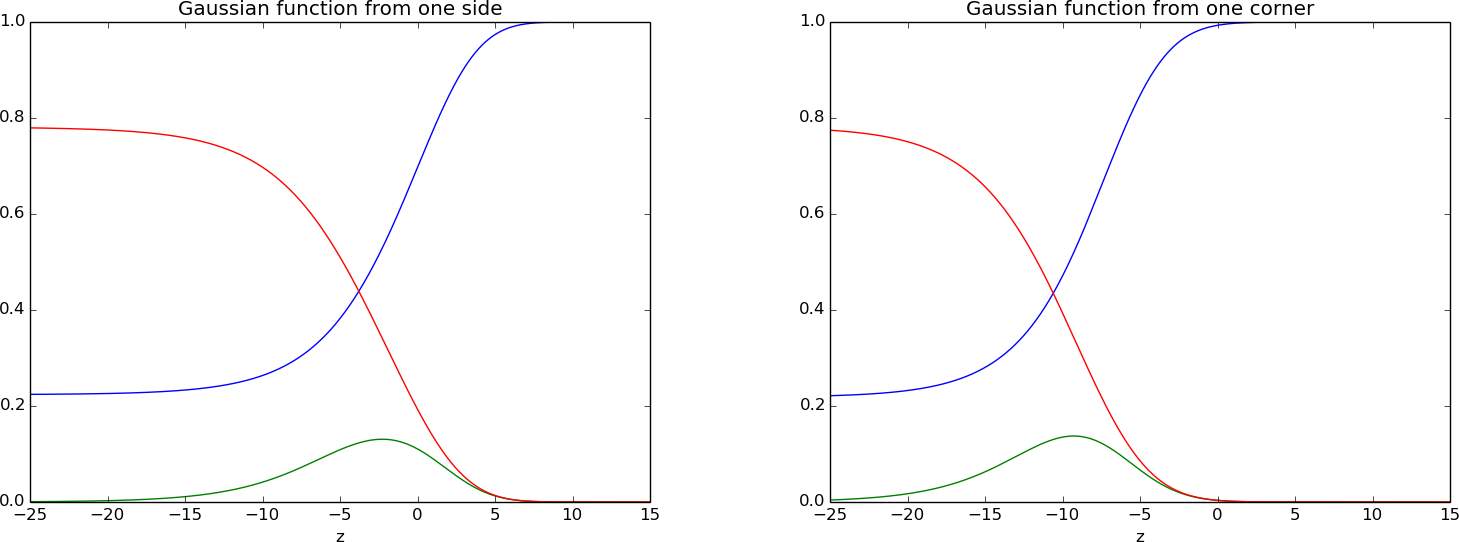
\includegraphics[width=0.8\linewidth]{plots/Trav_wave_2D.eps}}
  \caption{
  \label{fig:2D_trav_wave} Travelling wave measured at point (15,15) with two different initial values for the Infected class. The initial value is sat as a Gaussian line along (0,y) in the left plot and as a Gaussian point (0,0) in the right plot
  }
\end{figure}
%\clearpage % flush figures fig:2D_trav_wave


The shape of these two travelling waves are similar. The only difference is the time when the wave occur. The plot for 1D wave in fig(\ref{fig:1D_tw}) has the same shape. With a closer study, the area under the function can be measured for all three cases. The result can be seen in the table below.   

% 1D
% 1.4340793845
% 1.43143259034 dt = $1\cdot10^{-3}$, dx = 0.05
% 1.43195870243 dt = 0.0002, dx^2 = 0.000625
% 2D wave line:
% 1.43345609926 dt =0.0004, dx^2 =  0.0016
% 2D wave point:
1.43352971688

\begin{quote}
\begin{tabular}{ccc}
\hline
\multicolumn{1}{c}{ 1D wave } & \multicolumn{1}{c}{ 2D wave line } & \multicolumn{1}{c}{ 2D wave point } \\
\hline
1.43          & 1.43          & 1.43          \\
\hline
\end{tabular}
\end{quote}

\noindent
The area in all three cases are similar. The size and shape will not be affected based on the expansion from 1D to 2D. But by studying the figure(\ref{fig:2D_trav_wave}), the waves occur at different time in the two 2D simulations. This is caused by the distance from the start position for the Gaussian wave. The first subplot that starts with a Gaussian function along the $x=0$ axis, gets a wave of infected wash along the x axis. This can be seen as a wave on the beach. Everyone that have the same distance from the ocean will be hit simultaneously. The travelling wave for the 1D simulation and the first subplot occur at the same time, because they are measured at the same distance from the starting point. The last plot is also measured at (15,15), but occur later. Since the wave starts at point (0,0), the distance to (15,15) is 21.21. This means that the wave will start about 6 time steps later. This is also reasonable by looking at the plot.    


\paragraph{Change in initial flow.}
Another test that can be done to the travelling wave, is to check if the size of the initial wave will affect the travelling wave. The simulation is run with the same parameter as for the three simulations above and the only difference is the initial value for the infected group. The Gaussian wave of infected are placed a point (0,0) as for right subplot in figure(\ref{fig:2D_trav_wave}).The simulation can be seen in figure(\ref{fig:initial_value}).  
% Volume ordinary = 0.3141592653589793
% Volume extreme = 157.07963267948966
% Volume under graph 1.43345609926

\begin{figure}[ht]
  \centerline{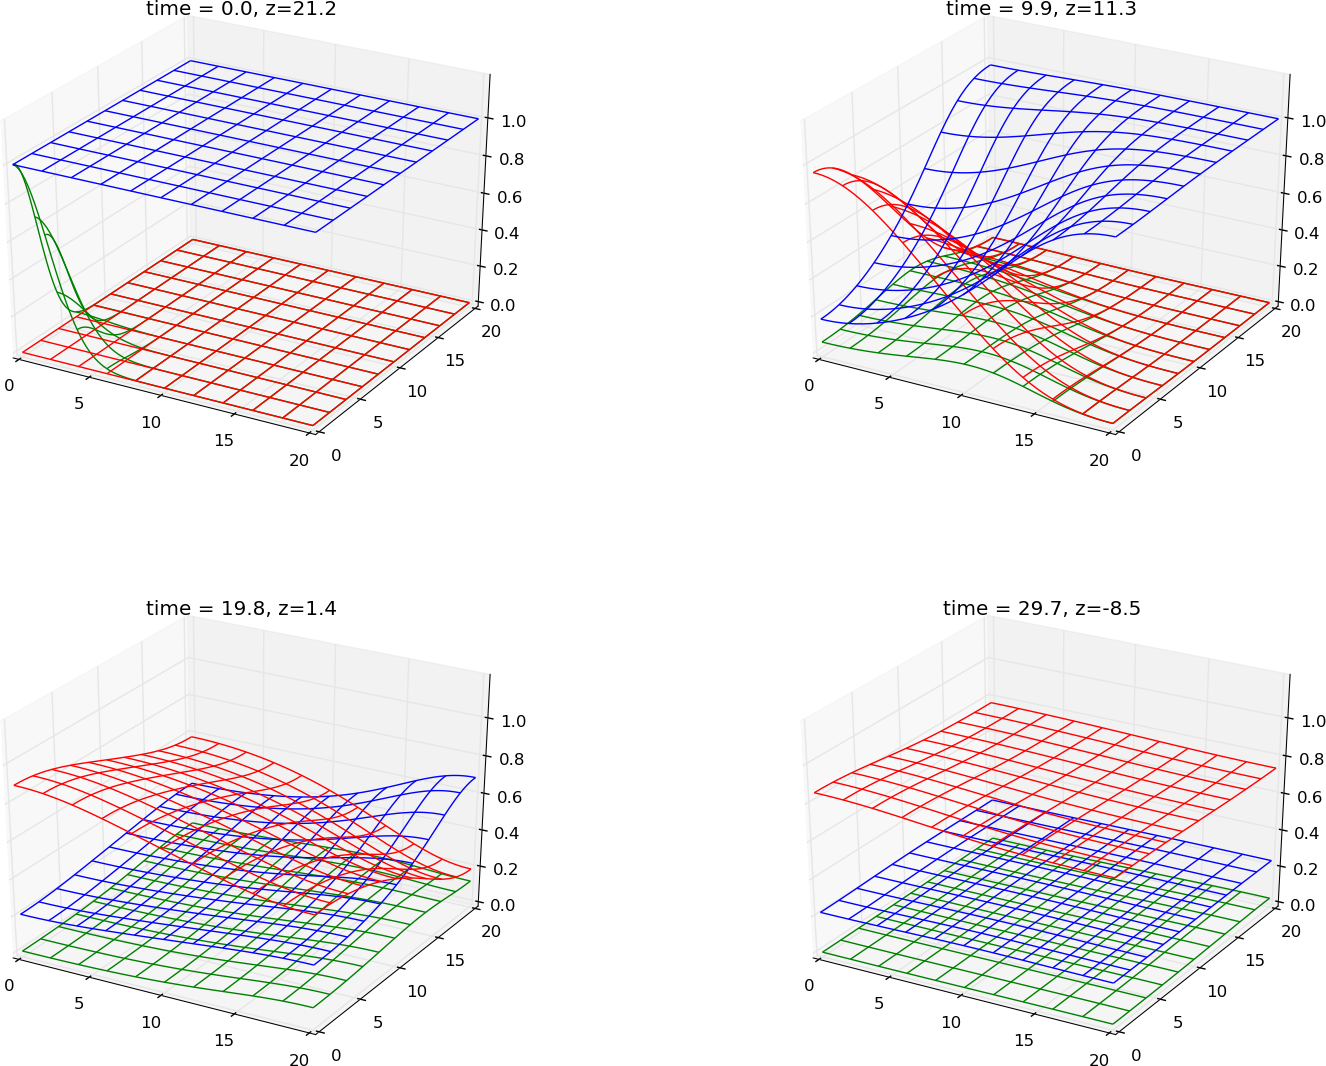
\includegraphics[width=0.8\linewidth]{plots/2D_initial_variable_sub.eps}}
  \caption{
  \label{fig:initial_value} A major flow of infected spread outwards the field. After a certain time, the wave has past the area and the number in each class stabilize.
  }
\end{figure}
%\clearpage % flush figures fig:initial_value


By measuring the travelling wave at (15,15), the size and shape can be compared with the second subplot in figure(\ref{fig:2D_trav_wave}). This is done in figure(\ref{fig:initial_trav_wave}).


\begin{figure}[ht]
  \centerline{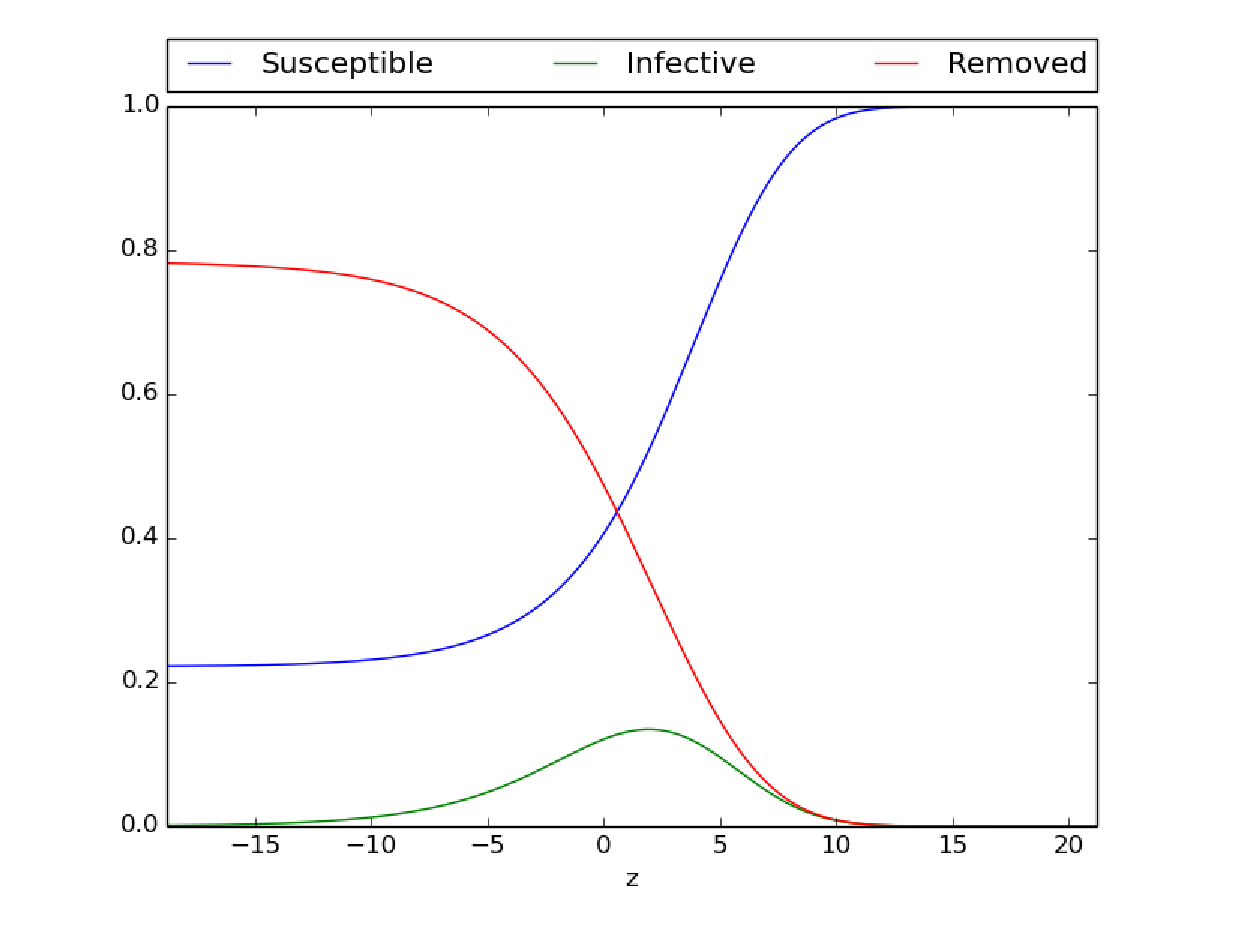
\includegraphics[width=0.8\linewidth]{plots/TW_2D_initial_z_lambda_0_5.eps}}
  \caption{
  \label{fig:initial_trav_wave} The travelling wave with a major increase of infected at the initial time.
  }
\end{figure}
%\clearpage % flush figures fig:initial_trav_wave


The figure(\ref{fig:initial_trav_wave}) shows a similar size and shape as for the other simulations run earlier. By increasing the initial value, the size of the travelling wave cannot be affected. But there is a difference in the time when the wave occur. In this simulation where the initial value is higher, the travelling wave reaches the measuring point (15,15) earlier. This can be explained by the idea of a ball dropped from height. If the ball is released or thrown to the ground, will only affect the acceleration of the ball, but not the terminal velocity. After a certain time the released ball and the thrown ball will reach the same maximum speed. This is also the case for the speed of the travelling wave. 
\paragraph{Change in lambda.}
The one thing that affects the speed and size, is the $\lambda$ variable in the PDE system(\ref{eq:simple_non_PDE}). This $\lambda$ is a combination of $a$, which controls deaths among infected, $r$, which control the number of infected in a meeting between an infected and a susceptible. The last parameter in $\lambda$ is the concentration of Susceptible. By changing this parameter, the travelling wave will change in both size and shape. In figure(\ref{fig:change_lambda}), the simulation is run with four different values of $\lambda$.


\begin{figure}[ht]
  \centerline{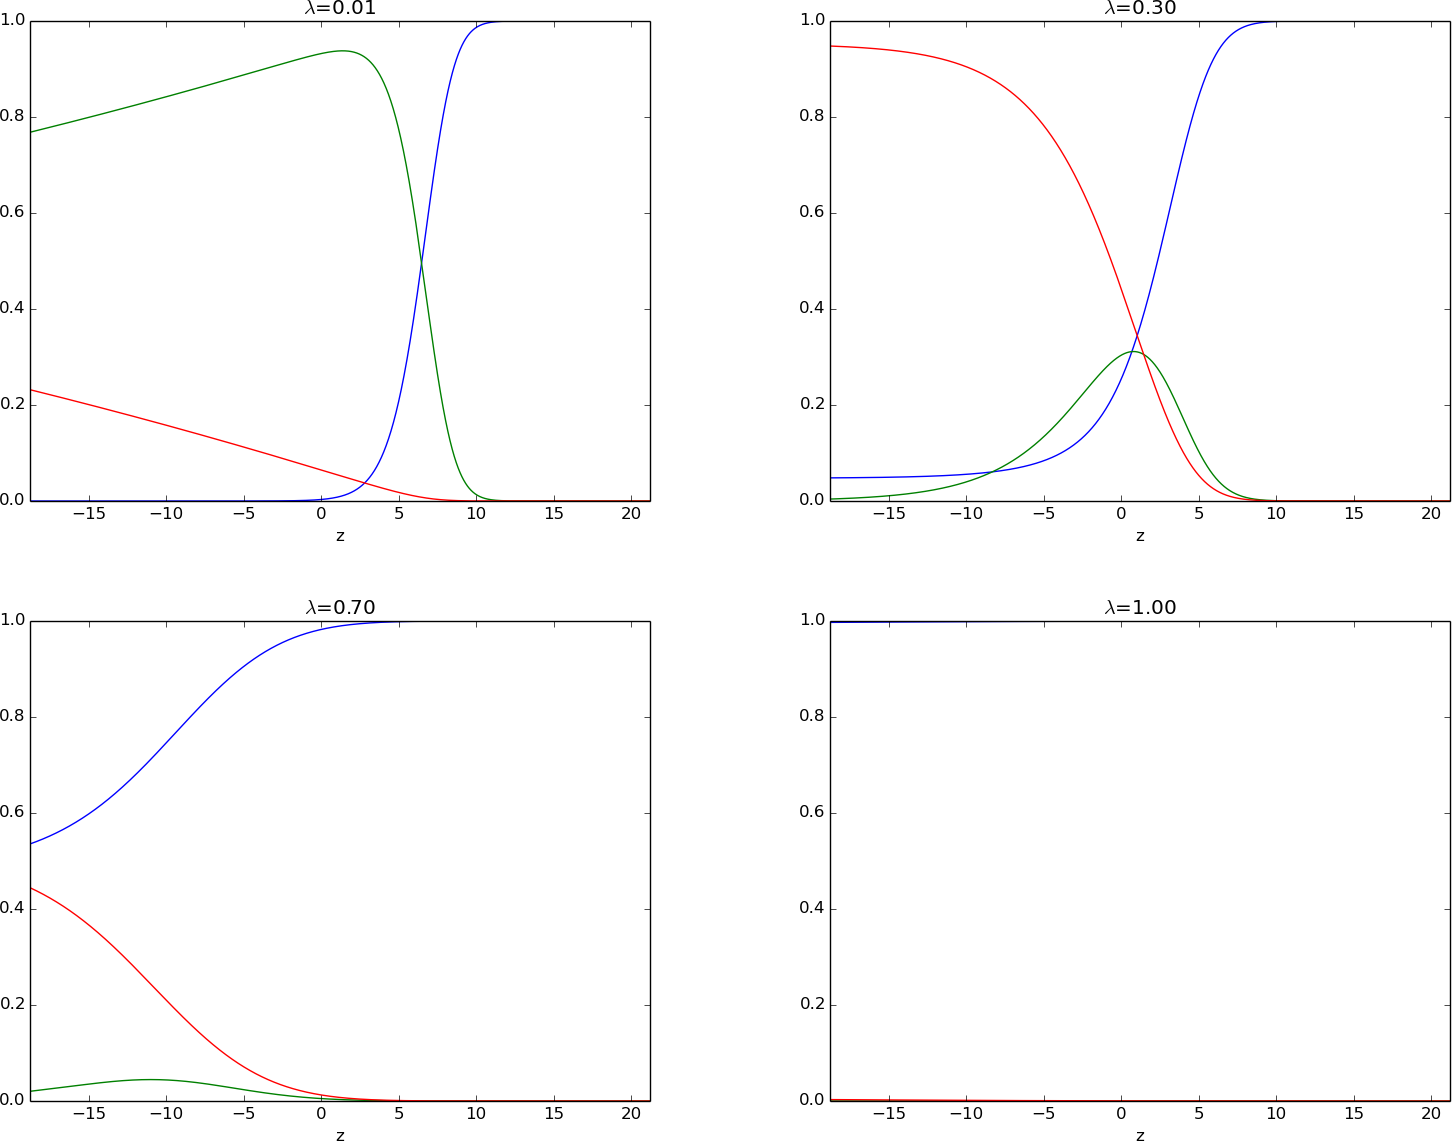
\includegraphics[width=0.9\linewidth]{plots/2D_lambda_variable.eps}}
  \caption{
  \label{fig:change_lambda} The travelling wave simulated with $\lambda$ values in the range of 0.01 to 1
  }
\end{figure}
%\clearpage % flush figures fig:change_lambda


To understand the result in figure(\ref{fig:change_lambda}), the $\lambda $ function can be study,
\begin{equation} \label{eq:lambda}
 \lambda =\frac{a}{rS_0},
\end{equation}
When $\lambda \rightarrow 0$, this cause a major and aggressive travelling wave. In figure(\ref{fig:change_lambda}), $\lambda$ is run with the value 0.01 in the first subplot. This result in a travelling wave of infected that eradicates the number of Susceptible in a short time. The wave stars decreasing when all Susceptible are infected. By looking at the equation(\ref{eq:lambda}), a small value is caused by a small $a$ compared to $r$ and $S_0$. If $a$ is low, this result in few deaths/immune in the infected class. This means that this class will grow and be able to infect even more humans from the Susceptible class. The same thing will happen if $r$ is large. A result of this will cause an aggressive disease that will infect major part of the population. The same result will happen if $S_0$ is large. Then there are several possible humans to infect. Therefore a outburst of a disease is more critically in a city than in the wilderness far from other humans.
\\
\\
If $\lambda$ increases above 1, the disease will not be able to spread. Then the number of infected will decrease, since the number of dead/immune infected are higher than the infected susceptible. After a certain time, the number of infected will die out. If $\lambda$ stays at 1, the number of infected will be equal the whole time. 

\section{Epidemic in an English Boarding School 1978}
I the previous chapter an example from the English boarding school was presented. This example was based on the book from J.D Murray and was modeled for a ODE system. By using the parameters a similar result should appear for the PDE system. The school had 763 students where one of the students brought with him a disease back to the school. The following number was used for the ODE system in chapter one. $N=763, S_0=762,I_0=1,R_0=0,\rho=202$ and $r = 2.18\cdot 10^{-3}$. 
\\
\\
The first simulation that is done on the PDE system is produced with an uniform distributed concentration of the three classes all over the area. A person has a given volume of one cubic. The total volume of the whole group is spread over the area. The area is sat to be 10 x 10, which means that the height of one person will be $1/100$. Since the Infected group only consist of one person, the total height will be 0.01 for the whole area. The Susceptible group consist of 762 students and the total height in each point will be 7.62. The simulation can be seen in the Appendix. 
\\
\\
The results from figure(\ref{fig:british_number}) are equal with the result from the ODE system modeled in the previous chapter.This can be seen in (\ref{table:british_number_table})  This is as expected since the diffusion term i negligible in this system and that it in reality is group of separate ODE systems modeled over an area.


\begin{figure}[ht]
  \centerline{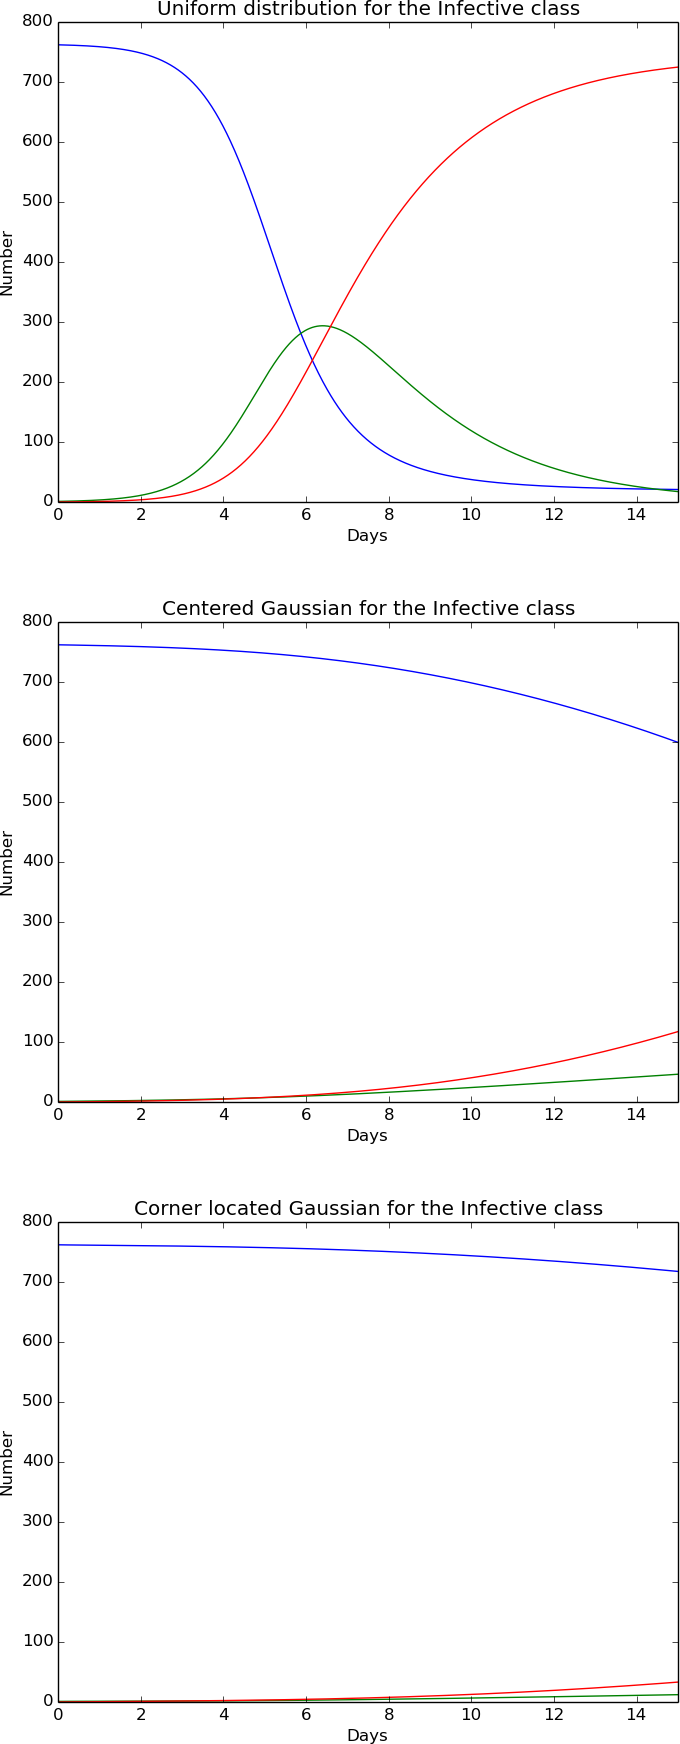
\includegraphics[width=0.8\linewidth]{plots/british_number.eps}}
  \caption{
  \label{fig:british_number} English Boarding School modeled over a uniform distributed area.
  }
\end{figure}
%\clearpage % flush figures fig:british_number


\label{table:british_number_table}

\begin{quote}
\begin{tabular}{ccccc}
\hline
\multicolumn{1}{c}{  } & \multicolumn{1}{c}{ ODE system } & \multicolumn{1}{c}{ PDE uniform dist } & \multicolumn{1}{c}{ PDE center } & \multicolumn{1}{c}{ PDE corner } \\
\hline
5 Days              & -----------         & ------------------- & -----------         & -----------         \\
\hline
Susceptible         & 444.62              & 444.62              & 748.03              & 757.33              \\
Infective           & 209.56              & 209.56              & 7.36                & 2.35                \\
Removed             & 108.82              & 108.82              & 7.60                & 3.32                \\
\hline
10 Days             & -----------         & ------------------- & -----------         & -----------         \\
\hline
Susceptible         & 37.59               & 37.59               & 697.71              & 743.58              \\
Infective           & 117.59              & 117.59              & 24.43               & 6.66                \\
Removed             & 607.82              & 607.82              & 40.86               & 12.76               \\
\hline
15 Days             & -----------         & ------------------- & -----------         & -----------         \\
\hline
Susceptible         & 21.09               & 21.09               & 597.01              & 717.02              \\
Infective           & 17.30               & 17.30               & 46.96               & 12.37               \\
Removed             & 724.62              & 724.62              & 119.03              & 33.61               \\
\hline
\end{tabular}
\end{quote}

\noindent
% dx = 0.04
% dx^2 = 1.6E-3
% ODE = 1.5E-4

\paragraph{Introducing a Gaussian distribution of infective.}
A reasonable assumption to make is that a person is not able to be evenly distributed over an area. In this example with only one infected student, the chance of being infected increase as closer you get to the infected student. To check in this affect the result, the volume of student is placed as a gauss function in the center of the schoolyard at initial time. The height is sat to 1 and the volume of the Gauss function is sat to 1 cubic. The simulation can be seen in figure(\ref{fig:gauss_sub}) and the total total amount of students can be be seen in figure(\ref{fig:british_number}).


\begin{figure}[ht]
  \centerline{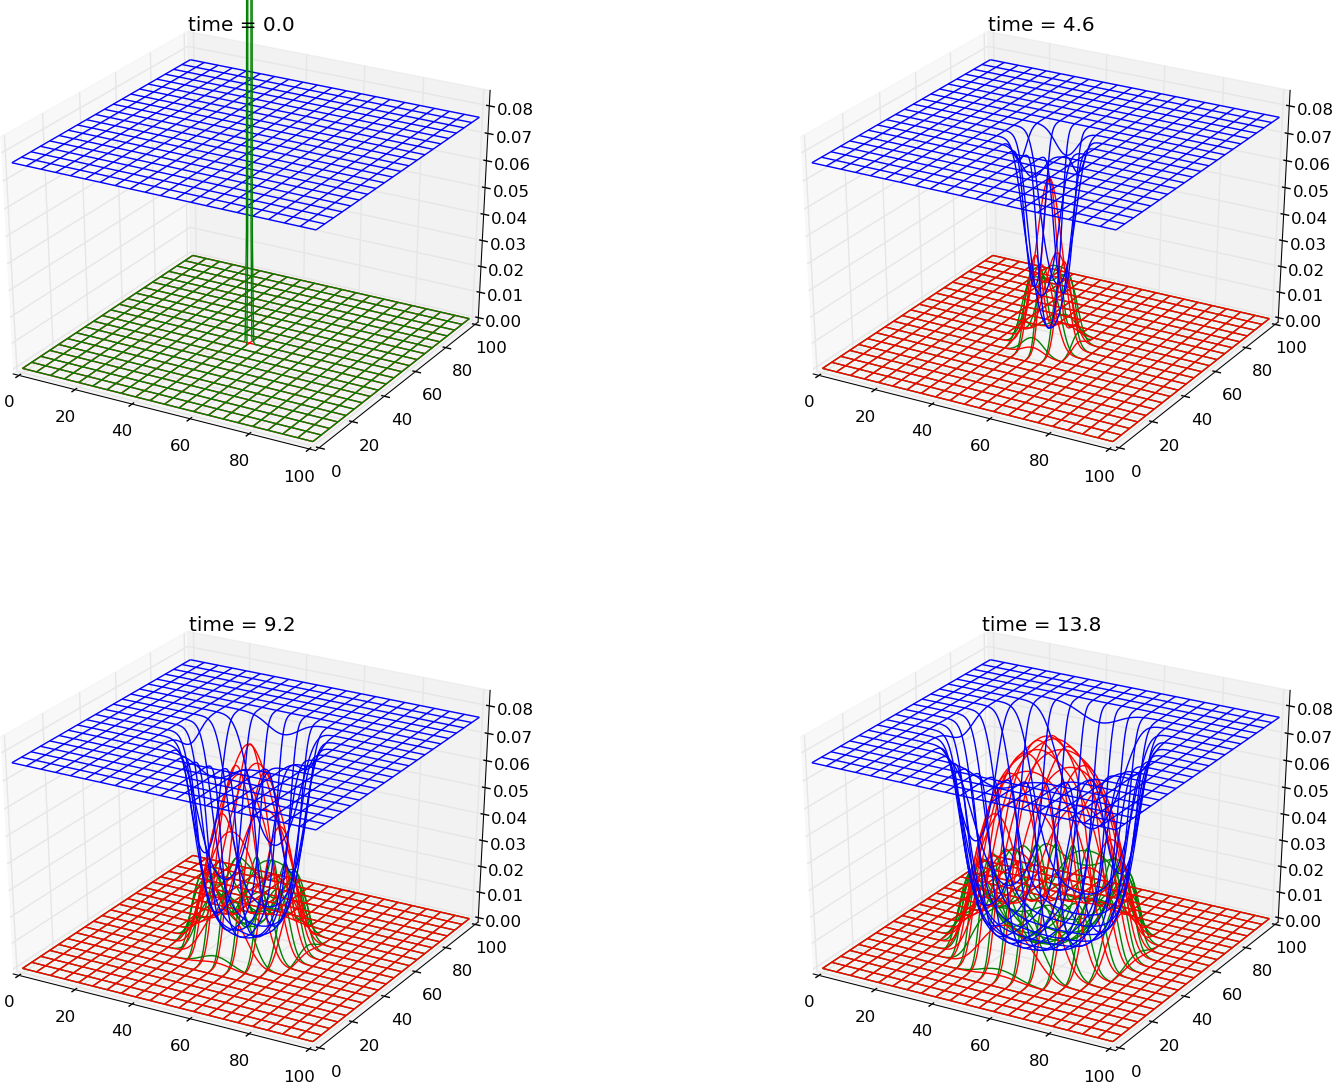
\includegraphics[width=0.8\linewidth]{plots/2D_british_school_gauss_sub.eps}}
  \caption{
  \label{fig:gauss_sub}
  }
\end{figure}
%\clearpage % flush figures fig:gauss_sub


\\
\\
By comparing the result from the uniform distributed PDE system and this simulation there are some interesting results. While the only difference between the two simulations is the placement of the infective. And this change has a major impact. Since the only one that can be infected are the students close to the infective, it restrict the spread of the epidemic. But the chance of getting infected in this area is major. The figure(\ref{fig:gauss_sub}) shows that the amount of infective quickly grow in the center, where the infected one was placed. The last subplot also show  that the amount of removed in the center are closed to the maximum of the initial value of Susceptible. While the students along the boundary of the school seems to be unaffected after 15 days. This simulation show that the placement of the infective has a major role in the simulation.
\\
\\
The placement of the Infective class also has an effect on the spread of the disease. The last column in (\ref{table:british_number_table}) describe a simulation where the Gaussian function is placed in the corner(0,0). The total volume of the function is increased to 4 since only a quarter of the function is placed in the area. The table shows that the total number of infected is lower than for the centered placed Gaussian. This infected student is only able to spread the disease to a quarter of the population compared with the infected one in the center. The simulation can be seen in the Appendix.
\\
\\
If the simulations are run for a longer time, the difference in each class will decrease. After 100 days there will be about 18 Susceptible students left in the uniform distributed group, while there will be about 25 students in both of the Gaussian groups. The simulations can be seen in the Appendix.

% !split
\section{Zombiefication}
The previous chapter studied a ODE system which was used to calculate the results of the TV series \emph{Walking Dead}. This model was based on the system from LMR and was developed with an extra term in the  phase \emph{counter attack}. The following system that was used in chapter \emph{Epidemic models} can be expand with a diffusion term in each class. The PDE system can be seen in eq(\ref{eq:seland_model})  

\begin{align*} \label{eq:seland_model}
\frac{\partial S}{\partial t} =& \Sigma -(\beta+\mu \omega(t))SZ - \delta_SS +D_s\nabla^2 S \\
\frac{\partial I}{\partial t} =& (\beta+\mu \omega(t))SZ - \varrho I - D_i\delta_II+\nabla^2 I\\
\frac{\partial Z}{\partial t} =& \varrho I- (\alpha+\omega(t))SZ + \zeta R+D_z\nabla^2 Z\\
\frac{\partial R}{\partial t} =& \delta_SS +\delta_II -\zeta R + (\alpha+\omega(t))SZ+D_r\nabla^2 R 
\end{align*}
By discretize this with Forward Euler in time and Crank Nicolson in space as for the SIR model(\ref{eq:SIR_disc}), the system can be expressed
\begin{equation} \label{eq:SIZR_disc}
	\begin{aligned}
    \frac{S^{n+1}_{i,j}-S^n_{i,j}}{\Delta t} &= \Sigma - (\beta+\mu \omega(t))S^{n}_{i,j}Z^{n}_{i,j}- \delta_S S^{n}_{i,j}+\
        D_s\left(\frac{S^{n}_{i-1,j}-2S^{n}_{i,j}+S^{n}_{i+1,j}}{\Delta x^2}+\frac{S^{n}_{i,j-1}-2S^{n}_{i,j}+S^{n}_{i,j+1}}{\Delta y^2}\right) \\
    \frac{I^{n+1}_{i,j}-I^n_{i,j}}{\Delta t} &= (\beta+\mu \omega(t))S^{n}_{i,j}Z^{n}_{i,j}-\varrho I^{n}_{i,j}- \delta_I I^{n}_{i,j}+\
        D_i\left(\frac{I^{n}_{i-1,j}-2I^{n}_{i,j}+I^{n}_{i+1,j}}{\Delta x^2}+\frac{I^{n}_{i,j-1}-2I^{n}_{i,j}+I^{n}_{i,j+1}}{\Delta y^2}\right) \\
    \frac{Z^{n+1}_{i,j}-Z^n_{i,j}}{\Delta t} &= \varrho I^{n}_{i,j}-(\alpha+\omega(t))S^{n}_{i,j}Z^{n}_{i,j}+ \zeta R^{n}_{i,j}+\
        D_z\left(\frac{Z^{n}_{i-1,j}-2Z^{n}_{i,j}+Z^{n}_{i+1,j}}{\Delta x^2}+\frac{Z^{n}_{i,j-1}-2Z^{n}_{i,j}+Z^{n}_{i,j+1}}{\Delta y^2}\right) \\
    \frac{R^{n+1}_{i,j}-R^n_{i,j}}{\Delta t} &= \delta_S S^{n}_{i,j}+\delta_I I^{n}_{i,j}-\zeta R^{n}_{i,j}+(\alpha+\omega(t))S^{n}_{i,j}Z^{n}_{i,j}
        D_r\left(\frac{R^{n}_{i-1,j}-2R^{n}_{i,j}+R^{n}_{i+1,j}}{\Delta x^2}+\frac{R^{n}_{i,j-1}-2R^{n}_{i,j}+R^{n}_{i,j+1}}{\Delta y^2}\right) 
	\end{aligned}
\end{equation}
By setting the unknown on the left side and the known on the right, the following system can be computed
\begin{equation} \label{eq:SIZR_disc2}
	\begin{aligned}
    S^{n+1}_{i,j} &= S^n_{i,j} + \Delta t \left( \Sigma - (\beta+\mu \omega(t))S^{n}_{i,j}Z^{n}_{i,j}- \delta_S S^{n}_{i,j}+\
        D_s\left(\frac{S^{n}_{i-1,j}-2S^{n}_{i,j}+S^{n}_{i+1,j}}{\Delta x^2}+\frac{S^{n}_{i,j-1}-2S^{n}_{i,j}+S^{n}_{i,j+1}}{\Delta y^2}\right)\right) \\
    I^{n+1}_{i,j} &= I^n_{i,j} + \Delta t \left((\beta+\mu \omega(t))S^{n}_{i,j}Z^{n}_{i,j}-\varrho I^{n}_{i,j}- \delta_I I^{n}_{i,j}+\
        D_i\left(\frac{I^{n}_{i-1,j}-2I^{n}_{i,j}+I^{n}_{i+1,j}}{\Delta x^2}+\frac{I^{n}_{i,j-1}-2I^{n}_{i,j}+I^{n}_{i,j+1}}{\Delta y^2}\right)\right) \\
    Z^{n+1}_{i,j} &= Z^n_{i,j} +\Delta t \left( \varrho I^{n}_{i,j}-(\alpha+\omega(t))S^{n}_{i,j}Z^{n}_{i,j}+ \zeta R^{n}_{i,j}+\
        D_z\left(\frac{Z^{n}_{i-1,j}-2Z^{n}_{i,j}+Z^{n}_{i+1,j}}{\Delta x^2}+\frac{Z^{n}_{i,j-1}-2Z^{n}_{i,j}+Z^{n}_{i,j+1}}{\Delta y^2}\right)\right) \\
    R^{n+1}_{i,j} &= R^n_{i,j} +\Delta t \left(\delta_S S^{n}_{i,j}+\delta_I I^{n}_{i,j}-\zeta R^{n}_{i,j}+(\alpha+\omega(t))S^{n}_{i,j}Z^{n}_{i,j}
        D_r\left(\frac{R^{n}_{i-1,j}-2R^{n}_{i,j}+R^{n}_{i+1,j}}{\Delta x^2}+\frac{R^{n}_{i,j-1}-2R^{n}_{i,j}+R^{n}_{i,j+1}}{\Delta y^2}\right)\right) 
	\end{aligned}
\end{equation}
To verify that the discretization has been done correct, a simulation with uniform distributed classes can be done. The result is the expected to be similar as for the ODE system in the previous chapter. A zombie attack can be separate into three different phases, explained in detail in the previous chapter. The first phase is short and is called the \emph{initial phase}. This is a condition where the humans are unfamiliar with the disease and behave quite naive to the disease. This result in a high chance of getting infected. The next phase is called \emph{Hysterical phase}. The humans are now more familiar with the situation and tries to avoid the infected ones. This result in a lower chance of getting infected. The last phase, which happens at the same time as the hysterical phase, is the counter attack. This phase is often started if the humans are attacked by zombies. The following parameter that was used for simulating the first episodes in \emph{Walking Dead} will also be used here. These can be seen in (\ref{table:param_val}). By compute the system for all three phases, the value in each phase can be compared with the ones from the ODE system in the previous chapter. This will give an indication if the discretization is done correct. 

\label{table:param_val}

\begin{quote}
\begin{tabular}{cccc}
\hline
\multicolumn{1}{c}{ parameter } & \multicolumn{1}{c}{ Initial phase } & \multicolumn{1}{c}{ hysterical phase } & \multicolumn{1}{c}{ counter attack } \\
\hline
$\beta$          & 0.01155          & 0.000011         & 0.00011          \\
$\varrho$        & 1.37             & 1.5              & 1.5              \\
$\alpha$         & 0.00044          & 0.000208         & 0.000208         \\
a                & 0                & 0                & 0.0073           \\
$\sigma$         & 0                & 0                & 0.005            \\
$\mu$            & 0                & 0                & 0.14             \\
\hline
\end{tabular}
\end{quote}

\noindent
The simulation in figure(\ref{fig:zombie_three_number}) seems to match the result from the ODE system. A closer check can be done by comparing the groups in each phase. This result can be seen in (\ref{table:compare_phases_zombie}) 


\begin{figure}[ht]
  \centerline{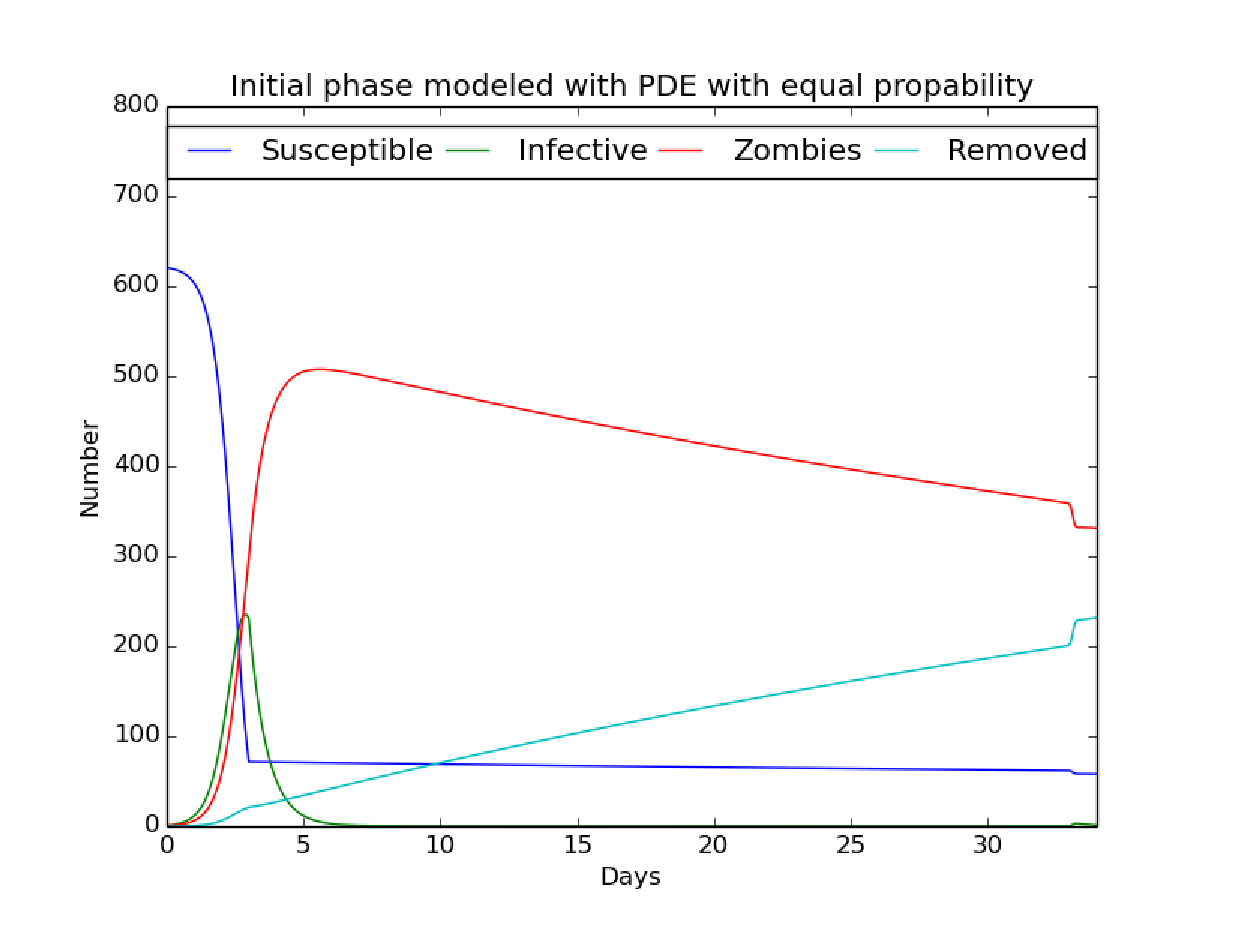
\includegraphics[width=0.8\linewidth]{plots/2D_zombie_three_phases_number.eps}}
  \caption{
  \label{fig:zombie_three_number} Same results as for the ODE system in the previous chapter
  }
\end{figure}
%\clearpage % flush figures fig:zombie_three_number


\label{table:compare_phases_zombie}

\begin{quote}
\begin{tabular}{cccc}
\hline
\multicolumn{1}{c}{  } & \multicolumn{1}{c}{ ODE system } & \multicolumn{1}{c}{ PDE uniform dist } & \multicolumn{1}{c}{ PDE gauss center } \\
\hline
Initial phase       & -----------         & ------------------- & ------------------- \\
\hline
Susceptible         & 71.3                & 71.5                & 81.12               \\
Infected            & 230.8               & 230.6               & 210.94              \\
Zombie              & 298.9               & 298.9               & 310.11              \\
Removed             & 21.0                & 21.0                & <:20.60             \\
\hline
Hysterical phase    & -----------         & ------------------- & ------------------- \\
\hline
Susceptible         & 61.6                & 61.8                & 70.55               \\
Infected            & 0.3                 & 0.3                 & 0.34                \\
Zombie              & 358.6               & 357.9               & 334.33              \\
Removed             & 201.5               & 202.0               & 217.56              \\
\hline
Counter attack      & -----------         & ------------------- & ------------------- \\
\hline
Susceptible         & 57.8                & 58.2                & 66.50               \\
Infected            & 1.2                 & 1.2                 & 1.23                \\
Zombie              & 331.8               & 331.1               & 305.86              \\
Removed             & 231.3               & 231.7               & 249.19              \\
\hline
\end{tabular}
\end{quote}

\noindent
These results shows that the PDE system gives the same result as for the ODE. The error can be controlled by decreasing the $\Delta t$ and $Delta x$ for the system. 

% #
% #
% #
% #



\paragraph{Variation in diffusion.}
% #
% #
% #
% #
% #
% #
% #
% #
% #
% #
% #
% #
% #
% #

\paragraph{Where does the infected one arises.}
In the previous section \emph{English boarding school}, the placement of the infected was proven to have a major influence on the result. But here the \emph{Susceptible} was uniformed distributed over the schoolyard. Based on the data from \emph{Walking Dead}, the amount in each class was based on three different places where Rick went by. Based on the TV series, it is hard to decide the geograpic distance between these three places. Therefore they have been placed with a certain distance from each other. The following simulation is done on a grid with size(20 x 20) with the following placement on the towns. Small(4,4) with size 21, middle(9,15) with size 200 and large(15,5) with size 400. Since these values was based on the humans and zombies seen in the series, these can be scaled up. The total population can be scaled up with 1000, so the large town can be seen as an area with a population of 400 000. The length can be measured in kilometre. Then the distance between the middle and large town will be 11.66 km. Compared to the distance between Oslo and Bærum(Sandvika) which is 15 km, the simulation can be seen as rough estimate of the area around Oslo.
\\
\\
The diffusion term describe the diffusion for each class. This can be seen as the speed of each group. If the diffusion constant is large, the flow towards equilibrium will go faster. The values have been sat as follows. 
\begin{itemize}
\item $D_s=1$, The \emph{Susceptible} has a basic moving speed. The other classes are based on the speed of a healthy human.

\item $D_i=0.5$, The \emph{Infected} are often injured caused by lately fights. This affect their moving speed

\item $D_z=0.9$, The average moving speed for a zombie. There are zombies with the moving speed of a human, but there are also cases where zombies edge them self forward with only one arm. This result in a major difference in speed and therefore a lower average speed for the zombies.

\item $D_r=0$, The removed are here seen as dead, therefore there are no moving speed.
\end{itemize}

\noindent
\\
\\
The parameters from (\ref{table:param_val}) will be used here and the three phases will be modeled as shown for the uniformed distributed PDE system. This will be done for three different simulations with similar initial value for the susceptible class. The initial value can be seen in figure(\ref{fig:initial_value_susceptible}) and are based on the data given above. The difference in the three different simulations will be the placement of the zombie at initial time. The zombie will be placed in center of the small, middle and large town.


\begin{figure}[ht]
  \centerline{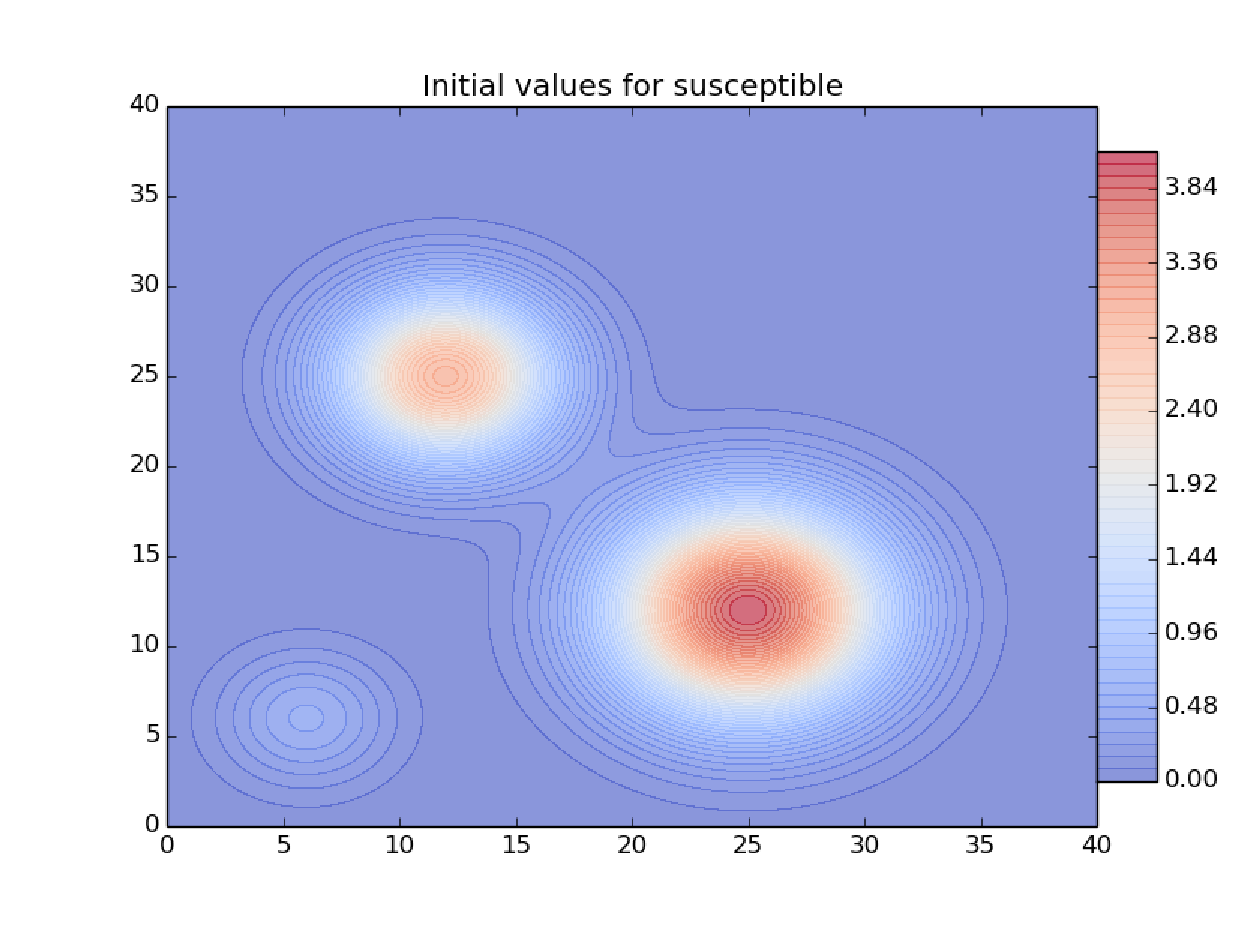
\includegraphics[width=0.8\linewidth]{plots/initial_value_susceptible.eps}}
  \caption{
  \label{fig:initial_value_susceptible}
  }
\end{figure}
%\clearpage % flush figures fig:initial_value_susceptible


The figure() shows the simulation where the zombie is placed in the small town. The four subplots are from the different phases that arise under a zombie attack. The different classes have the same color as introduced in figure(\ref{fig:zombie_three_number}). It is a challenge to separate the three groups \emph{Infected},*Zombie* and \emph{Removed}, since they all have a low value at initial time. The development of the amount can easier be seen in the figure(), which also shows the result from the placement in the middle and large group. Since the amount of \emph{Susceptible} is quite low in the small town where the Zombie arise, the disease is not able to infect to many before the society has moved to the next phase. Assuming that the broadcasting works okay for the first days. This result in a eradication of the disease in about a month. The table() shows that the number of zombies decrease towards zero after a month. 


\begin{center}  % inline figure
  \centerline{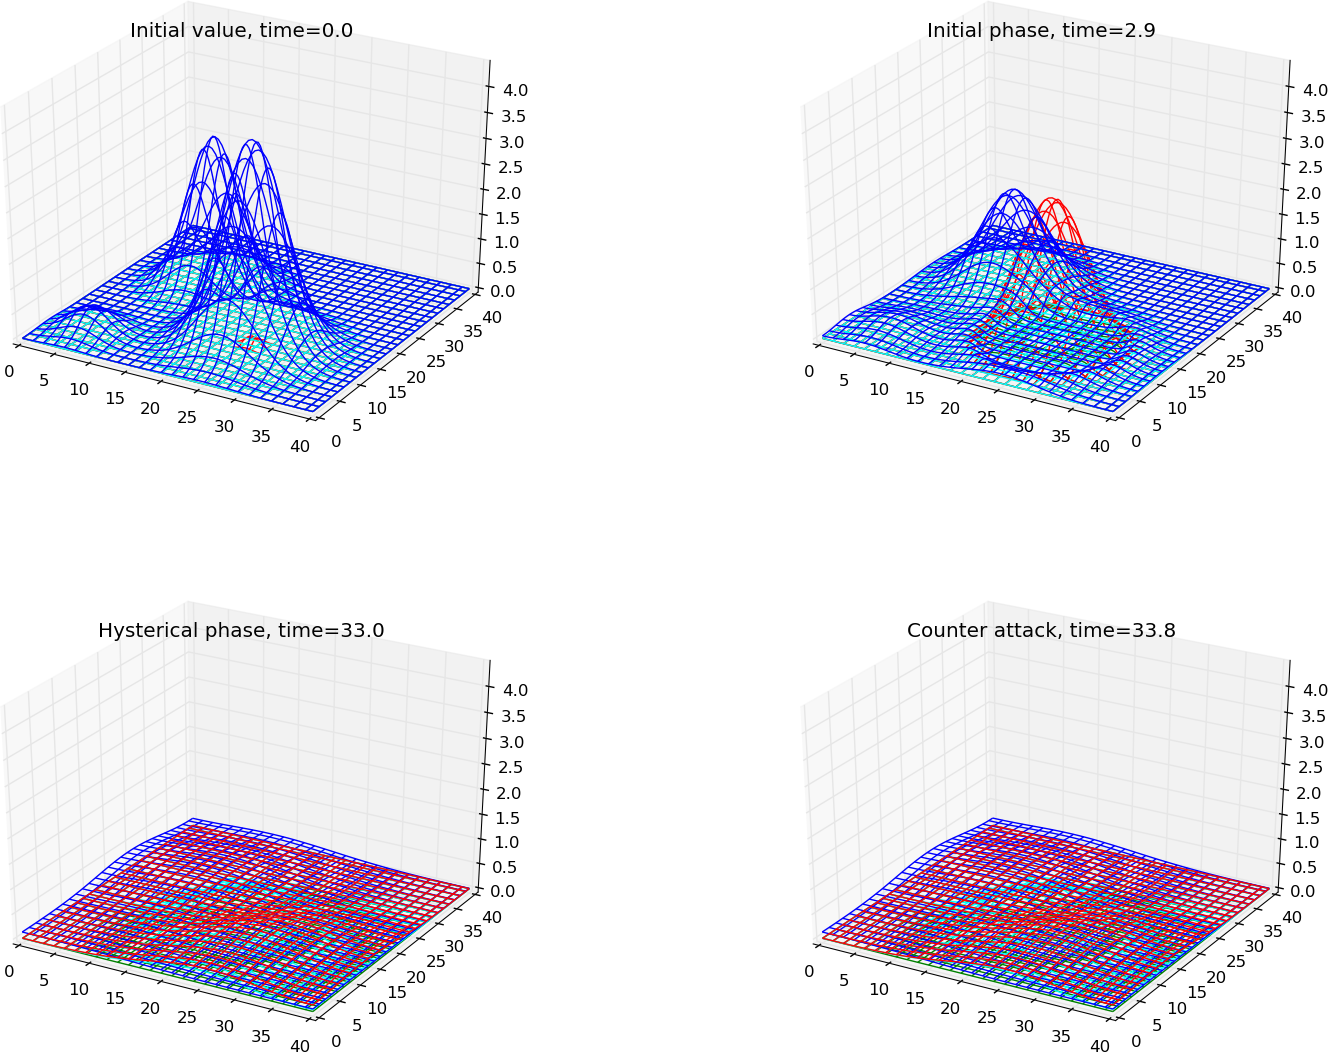
\includegraphics[width=0.8\linewidth]{plots/2D_zombie_three_phases_zombie_large_town_2_sub.eps}}
\end{center}


By placing the Zombie in the middle town, the amount of zombies increase to a much higher level. The amount can be seen as the second sub figure in figure(). The damages are higher and after a month the total population of \emph{Susceptible} will be reduced to around (300). The simulation can be seen in the Appendix. The last calculation done in the large town shows the major damages. Here the amount of zombies increase above the number of \emph{Susceptible}. The \emph{Infected} class also increase towards 100 around in the infected phase. This can be explained by the high number of meeting between susceptible and zombies. A plot that shows each class is produced for this simulation. This give a better overview of the concentration of the four groups during this simulation. Since the diffusion term for the \emph{Removed} group is sat to zero, the \emph{Removed} subplots gives an indication on the placement of the deaths. This seems to be grouped in the city. The amount of zombies also seems to be higher here. The major amount of \emph{Susceptible} are in the middle town. This area was able to avoid the damages from the initial phase.


The result from the uniformed distributed simulation still is much higher for the \emph{Zombie} class then for the large town. This shows that by using the parameters from the ODE system in a geographic area give no sense. A realistic assumption is that a zombie is restricted to a given area. Therefore the parameters will not be equal for all. The chance of getting infected is much higher if a susceptible is closed to an infected. There is also a greater chance of getting infected if the susceptible stay in a crowded area.


\begin{center}  % inline figure
  \centerline{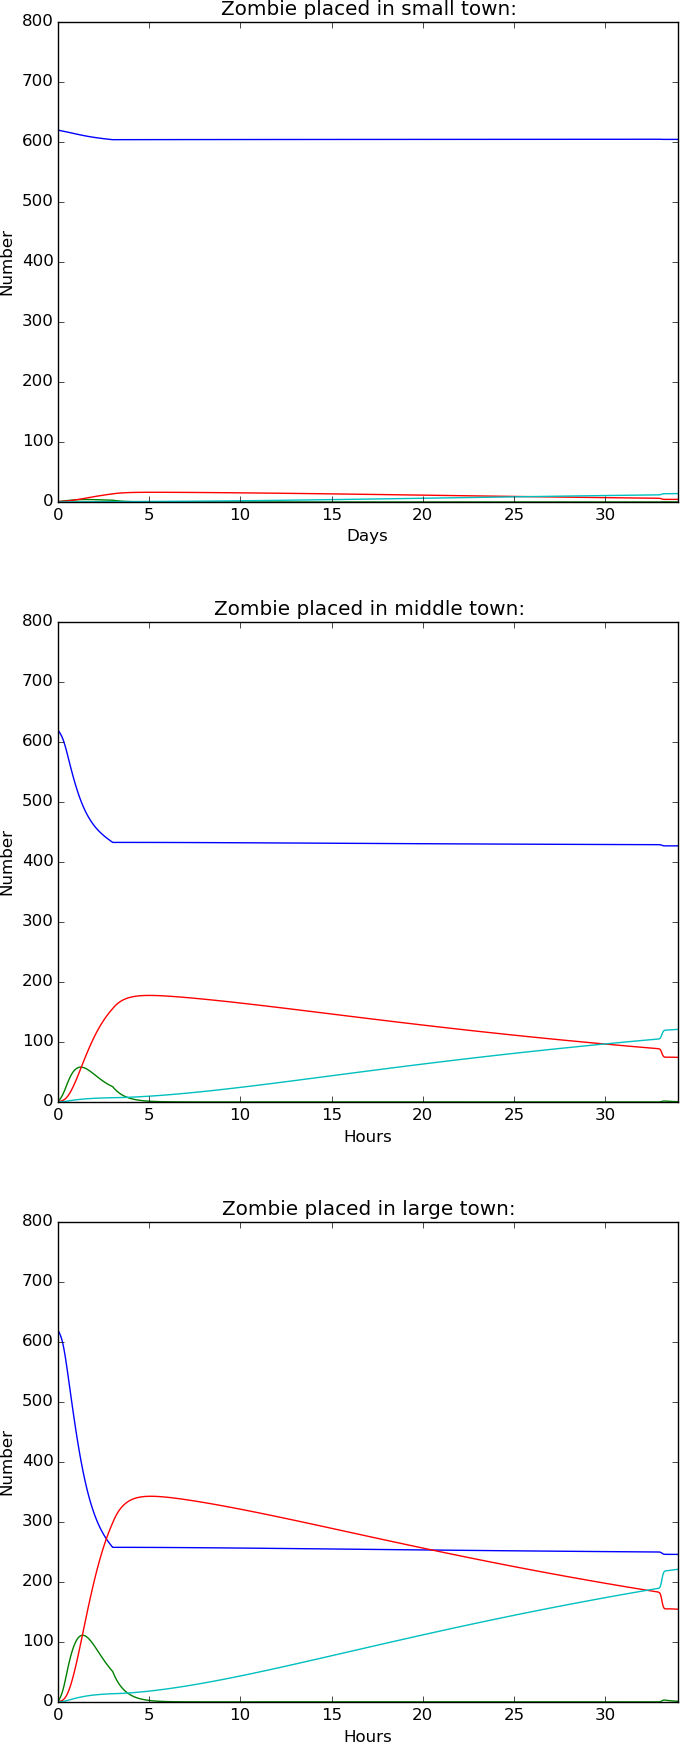
\includegraphics[width=0.8\linewidth]{plots/2D_compare_towns.eps}}
\end{center}


\label{table:compare_phases_zombie}

\begin{quote}
\begin{tabular}{cccc}
\hline
\multicolumn{1}{c}{  } & \multicolumn{1}{c}{ Small town } & \multicolumn{1}{c}{ Middle town } & \multicolumn{1}{c}{ Large } \\
\hline
Initial phase       & -----------         & ------------------- & ------------------- \\
\hline
Susceptible         & 603.74              & 433.22              & 259.20              \\
Infected            & 2.96                & 25.51               & 50.94               \\
Zombie              & 13.79               & 155.27              & 297.24              \\
Removed             & 0.66                & 7.16                & 13.78               \\
\hline
Hysterical phase    & -----------         & ------------------- & ------------------- \\
\hline
Susceptible         & 604.42              & 429.35              & 251.14              \\
Infected            & 0.03                & 0.18                & 0.35                \\
Zombie              & 6.25                & 87.31               & 178.45              \\
Removed             & 12.14               & 106.00              & 192.90              \\
\hline
Counter attack      & -----------         & ------------------- & ------------------- \\
\hline
Susceptible         & 604.21              & 427.45              & 247.33              \\
Infected            & 0.08                & 0.59                & 1.17                \\
Zombie              & 4.49                & 73.70               & 151.44              \\
Removed             & 14.11               & 121.16              & 222.96              \\
\hline
\end{tabular}
\end{quote}

\noindent
\subsection{Lock in different areas}

To model a realistic zombie attack, humans ability to think logic is crucial in the fight. The moving speed was presented as a factor in the previous section. Another important skill that the \emph{Susceptible} class hold, is the ability to decide if an area is safe. In the TV series \emph{Walking Dead}, the humans build barricades to keep the zombies outside. This give the \emph{Susceptible} class free areas where they can stay. This idea can be transfer to the PDE system by rewrite the system (\ref{eq:seland_model}) with spatial dependent diffusion term. The diffusion constant $D_u$ is now replaced with a diffusion function $\gamma_u(x)$ for $u= S,I,Z,R$ which is spatial discretized.

\begin{equation} \label{eq:seland_model_diff}
    \begin{aligned} 
    \frac{\partial S}{\partial t} =& \Sigma -(\beta+\mu \omega(t))SZ - \delta_SS +\nabla(\gamma_S(x) \nabla S) \\
    \frac{\partial I}{\partial t} =& (\beta+\mu \omega(t))SZ - \varrho I - D_i\delta_II+\nabla(\gamma_I(x) \nabla I)\\
    \frac{\partial Z}{\partial t} =& \varrho I- (\alpha+\omega(t))SZ + \zeta R+\nabla(\gamma_Z(x) \nabla Z)\\
    \frac{\partial R}{\partial t} =& \delta_SS +\delta_II -\zeta R + (\alpha+\omega(t))SZ+\nabla(\gamma_R(x) \nabla R) 
    \end{aligned}
\end{equation}

The difference for this system compared with (\ref{eq:seland_model}) is the diffusion term in each equation. The discretization can be shown for for a general $\gamma$. This will be similar for all classes. A Crank nicolson discretization is used in space.

\begin{equation} \label{eq:gamma}
    \begin{aligned}
    &=\nabla(\gamma(x) \nabla S) \\
    &=(\gamma(x) S_x)_x+(\gamma(x) S_y)_y \\
    &= \left(\gamma(x) \frac{S^{n}_{i+1/2,j}-S^{n}_{i-1/2,j}}{\Delta x}\right)_x+\left(\gamma(x) \frac{S^{n}_{i,j+1/2}-S^{n}_{i,j-1/2}}{\Delta y}\right)_y \\
    &= \left(\frac{\gamma(x_{i+1/2,j})(S^{n}_{i+1,j}-S^{n}_{i,j})-\gamma(x_{i-1/2,j})(S^{n}_{i,j}-S^{n}_{i-1,j})}{\Delta x^2}\right)+\left(\frac{\gamma(x_{i,j+1/2})(S^{n}_{i,j+1}-S^{n}_{i,j})-\gamma(x_{i,j-1/2})(S^{n}_{i,j}-S^{n}_{i,j-})}{\Delta y^2}\right)
    \end{aligned}
\end{equation}
Since the calculation is based on spatial points, the values inside the function of $\gamma$ need to be adjusted. This can be done by an aritmetic mean, which can be seen in eq(\ref{eq:arith_mean}). The writing $q_{i+1/2}$ is used for the function $q(x_{i+1/2})$ with $x_{i+1/2} = x_i + 1/2 \Delta x$
\begin{equation} \label{eq:arith_mean}
q_{i+1/2} \approx \frac{1}{2}(q_i +q_{i+1})
\end{equation}
This arithmetic mean can be inserted for all $\gamma$'s in the system.By cleaning up, the system can be expressed.
\begin{equation} \label{eq:SIZR_disc3}
	\begin{aligned}
    S^{n+1}_{i,j} &= S^n_{i,j} + \Delta t \left( \Sigma - (\beta+\mu \omega(t))S^{n}_{i,j}Z^{n}_{i,j}- \delta_S S^{n}_{i,j}+\
        \frac{1}{2\Delta x^2}\left(\gamma_S(x_{i-1,j})(S^{n}_{i-1,j}-S^{n}_{i,j})+\gamma_S(x_{i,j})(S^{n}_{i-1,j}-2S^{n}_{i,j}+S^{n}_{i+1,j})+\gamma_S(x_{i+1,j})(-S^{n}_{i,j}+S^{n}_{i+1,j})\right)+\
        \frac{1}{2\Delta y^2}\left(\gamma_S(x_{i,j-1})(S^{n}_{i,j-1}-S^{n}_{i,j})+\gamma_S(x_{i,j})(S^{n}_{i,j-1}-2S^{n}_{i,j}+S^{n}_{i,j+1})+\gamma_S(x_{i,j+1})(-S^{n}_{i,j}+S^{n}_{i,j+1})\right)\right)\\
    I^{n+1}_{i,j} &= I^n_{i,j} + \Delta t \left((\beta+\mu \omega(t))S^{n}_{i,j}Z^{n}_{i,j}-\varrho I^{n}_{i,j}- \delta_I I^{n}_{i,j}+\
        \frac{1}{2\Delta x^2}\left(\gamma_I(x_{i-1,j})(I^{n}_{i-1,j}-I^{n}_{i,j})+\gamma_I(x_{i,j})(I^{n}_{i-1,j}-2I^{n}_{i,j}+I^{n}_{i+1,j})+\gamma_I(x_{i+1,j})(-I^{n}_{i,j}+I^{n}_{i+1,j})\right)+\
        \frac{1}{2\Delta y^2}\left(\gamma_I(x_{i,j-1})(I^{n}_{i,j-1}-I^{n}_{i,j})+\gamma_I(x_{i,j})(I^{n}_{i,j-1}-2I^{n}_{i,j}+I^{n}_{i,j+1})+\gamma_I(x_{i,j+1})(-I^{n}_{i,j}+I^{n}_{i,j+1})\right)\right)\\
    Z^{n+1}_{i,j} &= Z^n_{i,j} +\Delta t \left( \varrho I^{n}_{i,j}-(\alpha+\omega(t))S^{n}_{i,j}Z^{n}_{i,j}+ \zeta R^{n}_{i,j}+\
        \frac{1}{2\Delta x^2}\left(\gamma_Z(x_{i-1,j})(Z^{n}_{i-1,j}-Z^{n}_{i,j})+\gamma_Z(x_{i,j})(Z^{n}_{i-1,j}-2Z^{n}_{i,j}+Z^{n}_{i+1,j})+\gamma_Z(x_{i+1,j})(-Z^{n}_{i,j}+Z^{n}_{i+1,j})\right)+\
        \frac{1}{2\Delta y^2}\left(\gamma_Z(x_{i,j-1})(Z^{n}_{i,j-1}-Z^{n}_{i,j})+\gamma_Z(x_{i,j})(Z^{n}_{i,j-1}-2Z^{n}_{i,j}+Z^{n}_{i,j+1})+\gamma_Z(x_{i,j+1})(-Z^{n}_{i,j}+Z^{n}_{i,j+1})\right)\right)\\
    R^{n+1}_{i,j} &= R^n_{i,j} +\Delta t \left(\delta_S S^{n}_{i,j}+\delta_I I^{n}_{i,j}-\zeta R^{n}_{i,j}+(\alpha+\omega(t))S^{n}_{i,j}Z^{n}_{i,j}\right)
	\end{aligned}
\end{equation}
The diffusion term for the \emph{Removed} class is take away, since dead people are not able to move. This system looks quite messy, but it is straight forward to calculate. All values on the right side are known values and the system is easy to solve. Now every point will has its own diffusion constant. This makes it easier to control the flow in each class. With a high diffusion constant, the diffusion will spread fast. When the diffusion constant goes towards zero, the flow will go towards a steady state. This will result in a set of ODE systems modeled for each point.
\paragraph{Ten minutes at Frederikkeplassen.}
Frederikkeplassen at the university is an area for an upcoming zombie attack. This simulation will try to model a ten minutes sequence with the diffusion parameter added in this section. Since students often learn and interact fast, they will only use three minutes before they realise the danger and goes into the \emph{Hysterical phase}. A map of Frederikkeplassen is used to define the safe and non save areas. The buildings are set as areas where only the \emph{Susceptible} are allowed to move. This is done by setting the diffusion constant to zero for the \emph{Zombie} and \emph{Infected} class. Since the buildings will be safe spots for the \emph{Susceptible}, an idea would be to express this in the diffusion term. This more difficult, since the concentrations in each class wants to go towards equilibrium. A way to delay this process is by setting the diffusion constant to be low in the buildings and high outside. This will result in a fast diffusion in the open areas and 



\begin{center}  % inline figure
  \centerline{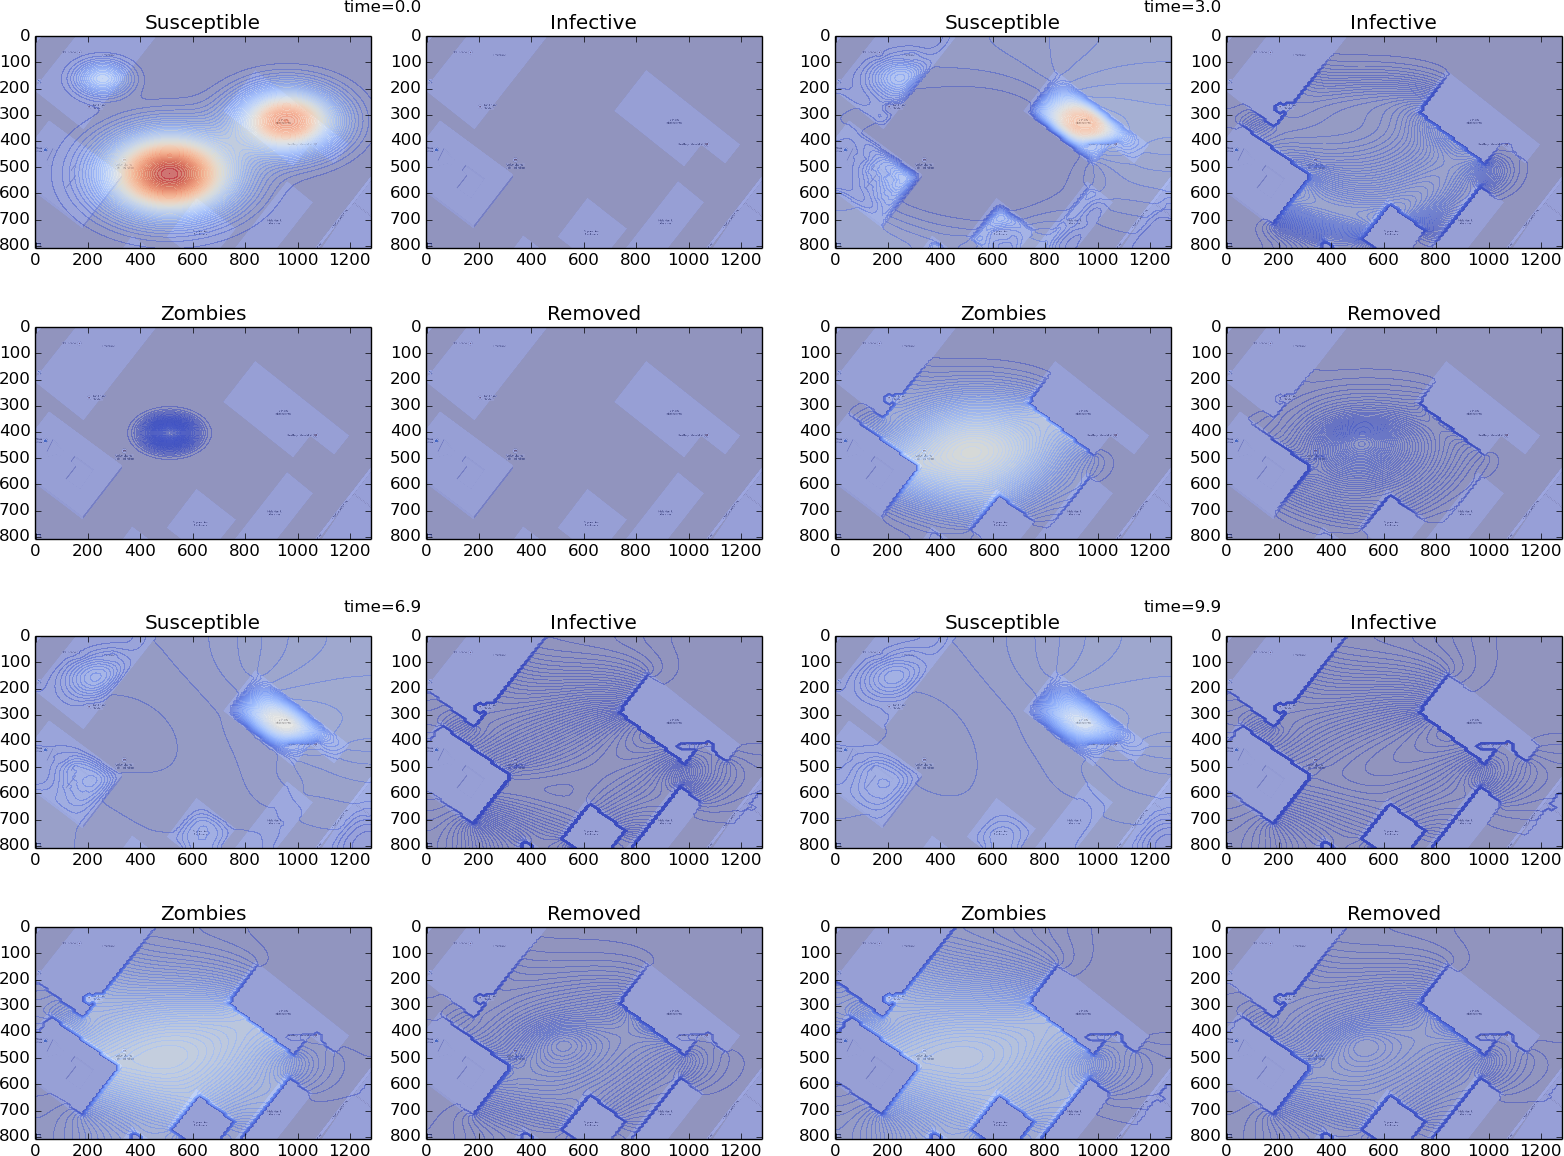
\includegraphics[width=0.8\linewidth]{plots/2D_Frederikke_contourf_sub.eps}}
\end{center}



\begin{center}  % inline figure
  \centerline{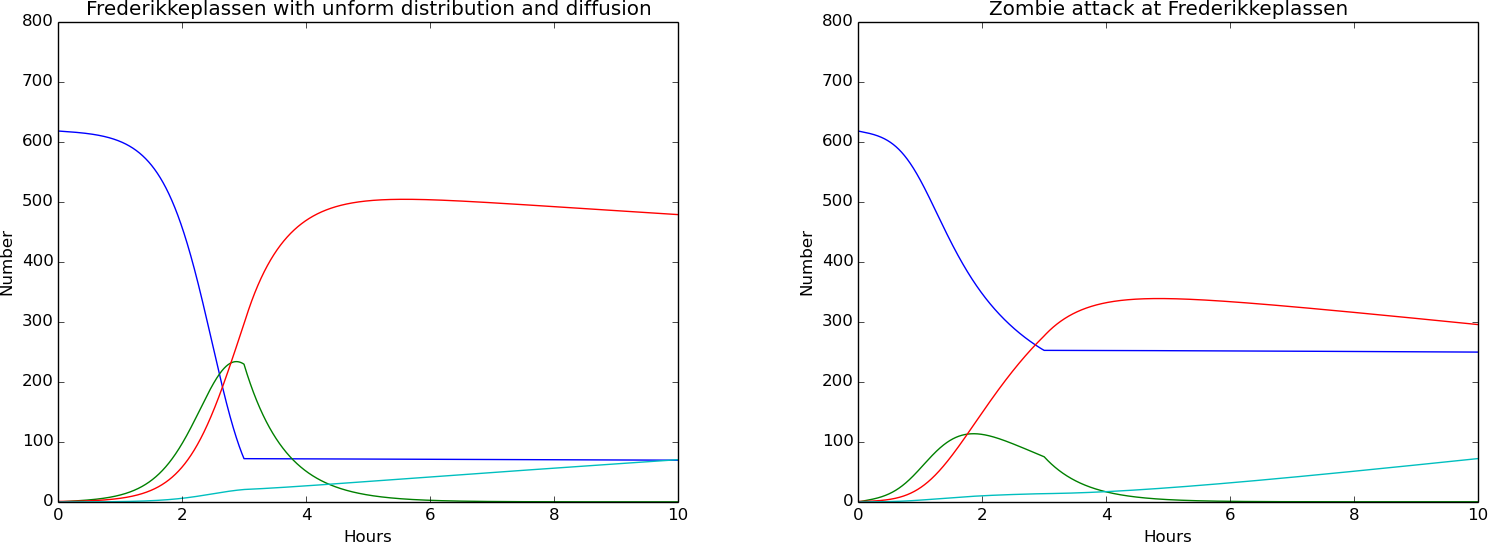
\includegraphics[width=0.8\linewidth]{plots/2D_compare_Frederikke.eps}}
\end{center}





% #
% #
-

\begin{quote}
\begin{tabular}{cccc}
\hline
\multicolumn{1}{c}{  } & \multicolumn{1}{c}{ Uniform distribution } & \multicolumn{1}{c}{ Free areas } & \multicolumn{1}{c}{ Random placement } \\
\hline
3 Minutes                   & --------------------------- & ---------------             & ----------------            \\
\hline
Susceptible                 & 72.23                       & 252.72                      & 524.77                      \\
Infected                    & 229.65                      & 75.69                       & 26.07                       \\
Zombie                      & 296.67                      & 276.55                      & 66.51                       \\
Removed                     & 20.84                       & 13.94                       & 3.66                        \\
\hline
7 Minutes                   & --------------------------- & ---------------             & ----------------            \\
\hline
Susceptible                 & 70.78                       & 251.35                      & 524.23                      \\
Infected                    & 0.83                        & 0.51                        & 0.20                        \\
Zombie                      & 498.72                      & 325.54                      & 81.88                       \\
Removed                     & 49.12                       & 41.26                       & 14.80                       \\
\hline
10 Minutes                  & --------------------------- & ---------------             & ----------------            \\
\hline
Susceptible                 & 69.69                       & 249.84                      & 523.61                      \\
Infected                    & 0.25                        & 0.38                        & 0.16                        \\
Zombie                      & 479.00                      & 295.71                      & 69.67                       \\
Removed                     & 70.55                       & 72.36                       & 27.77                       \\
\hline
\end{tabular}
\end{quote}

\noindent
\paragraph{random distribution.}
\begin{center}  % inline figure
  \centerline{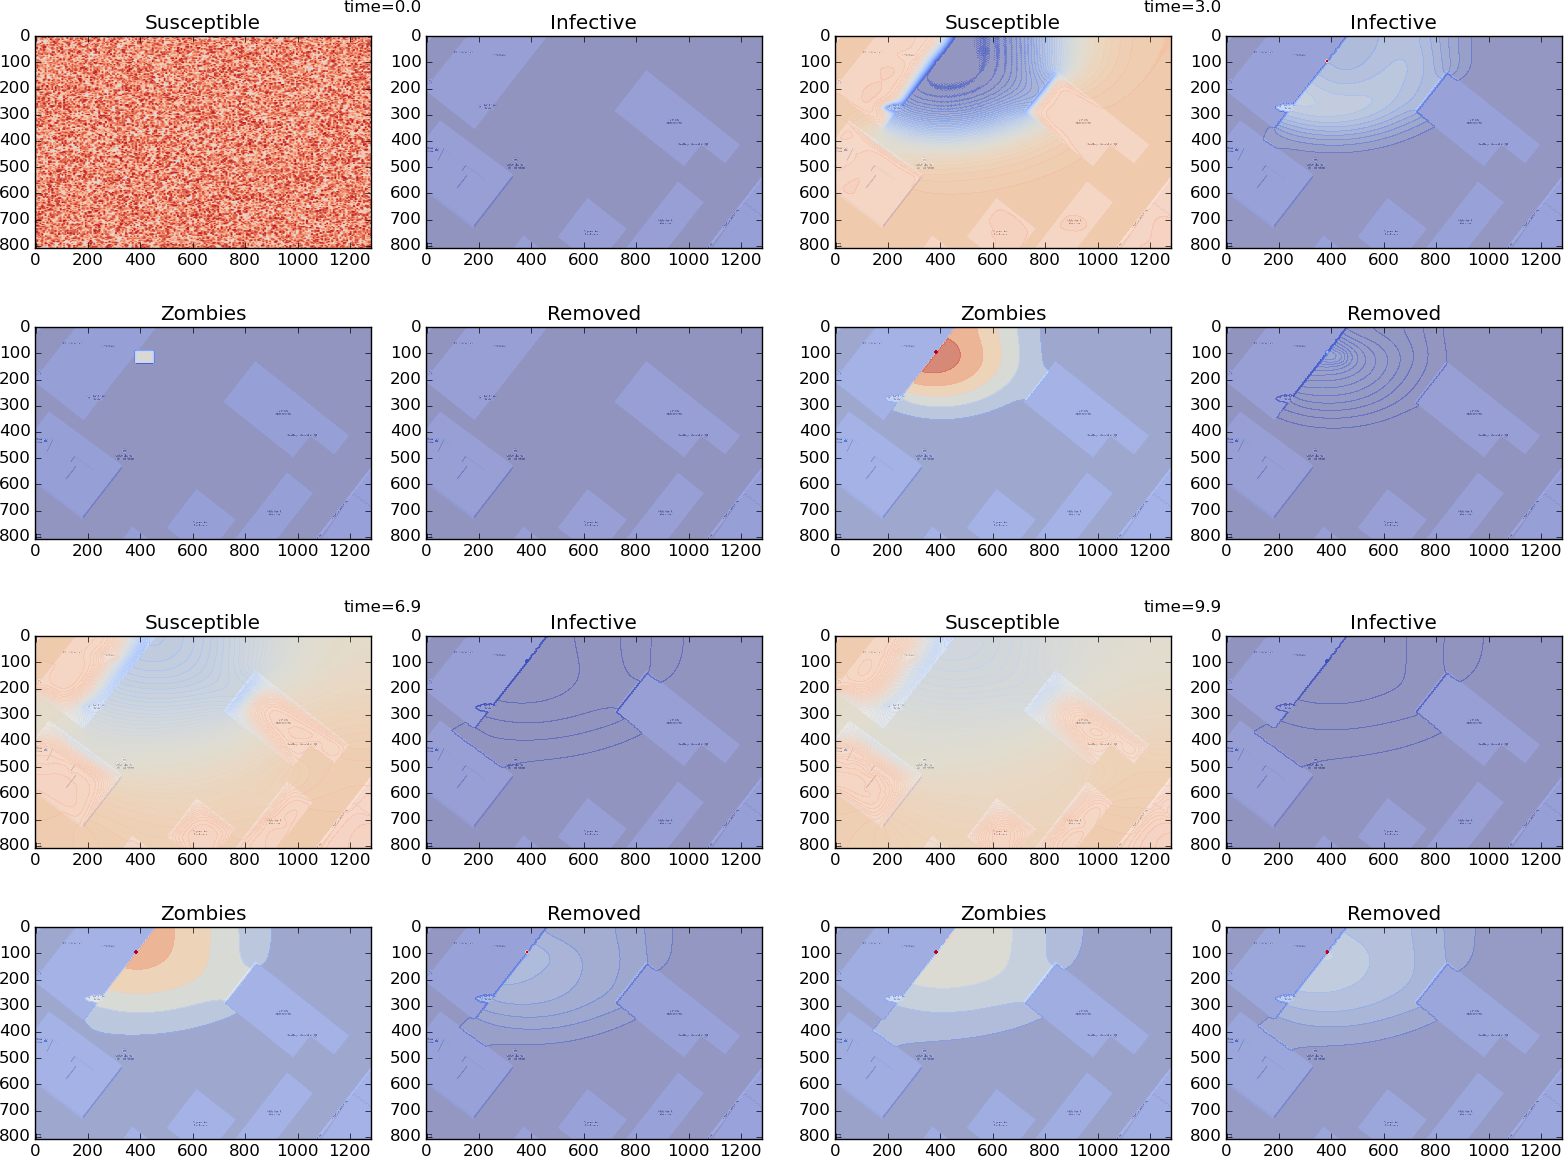
\includegraphics[width=0.8\linewidth]{plots/2D_Frederikke_random_contourf_sub.eps}}
\end{center}





% !split
\section{Appendix}
\subsection{Discretization}
\begin{equation} \label{eq:LMR_model}
	\begin{aligned} 
	\frac{dS}{dt} =& \Sigma -\beta SZ - \delta_SS + \nabla(\gamma_s(x)\nabla S) \\
	\frac{dI}{dt} =& \beta SZ - \varrho I - \delta_II+\nabla(\gamma_I(x)\nabla I)\\
	\frac{dZ}{dt} =& \varrho I- (\alpha+\omega(t))SZ + \zeta R+ \nabla(\gamma_Z(x)\nabla Z)\\
	\frac{dR}{dt} =& \delta_SS +\delta_II -\zeta R + (\alpha+\omega(t))SZ 
	\end{aligned}
\end{equation}
The calculations will be shown for the diffusion part in the first equation. This idea will be used for the whole system

\begin{equation}
	\begin{aligned}
	\frac{dS}{dt} =& \nabla(\gamma_s(x)\nabla S) \\
    \frac{S^{n+1}_{i,j}-S^n_{i,j}}{\Delta t} &= \left(\gamma(x_{i+1/2,j})\frac{S^{n}_{i-1,j}-2S^{n}_{i,j}+S^{n}_{i+1,j}}{\Delta x}+\frac{S^{n}_{i,j-1}-2S^{n}_{i,j}+S^{n}_{i,j+1}}{\Delta y}\right) 
	\end{aligned}
\end{equation}
\subsection{2D Gaussian function from x=0}


\begin{figure}[ht]
  \centerline{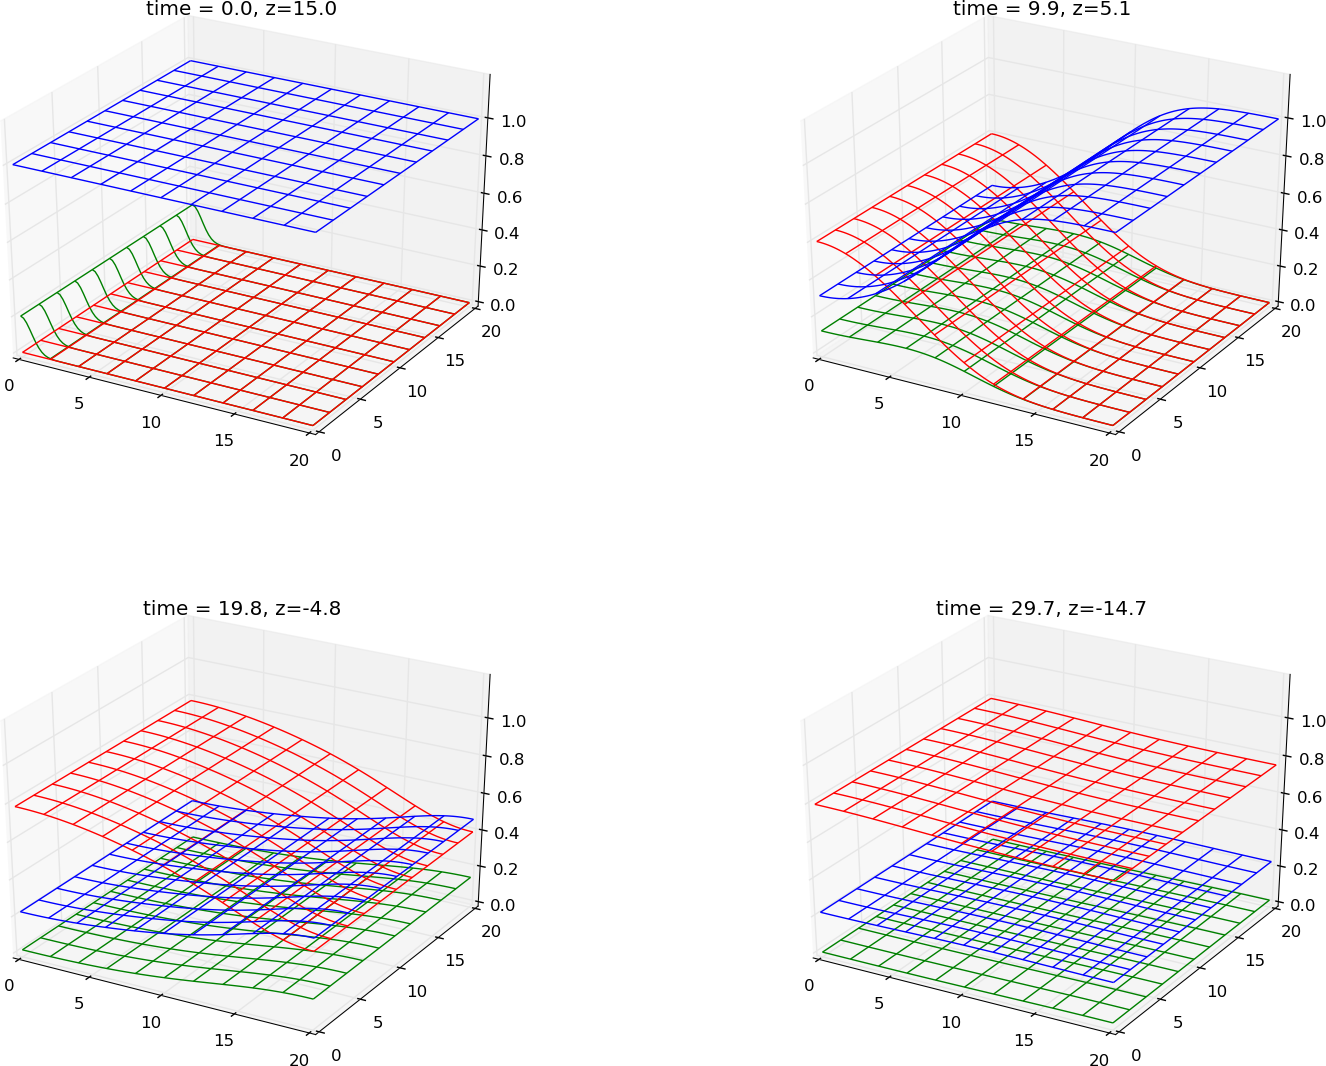
\includegraphics[width=0.8\linewidth]{plots/2D_gauss_sub.eps}}
  \caption{
  The PDE system (\ref{eq:simple_non_PDE}) simulated for a 2D system with $\lambda=0.5$. A gauss wave from $x=0$.
  }
\end{figure}
%\clearpage % flush figures 


\subsection{2D Gaussian function from x=0,y=0}


\begin{figure}[ht]
  \centerline{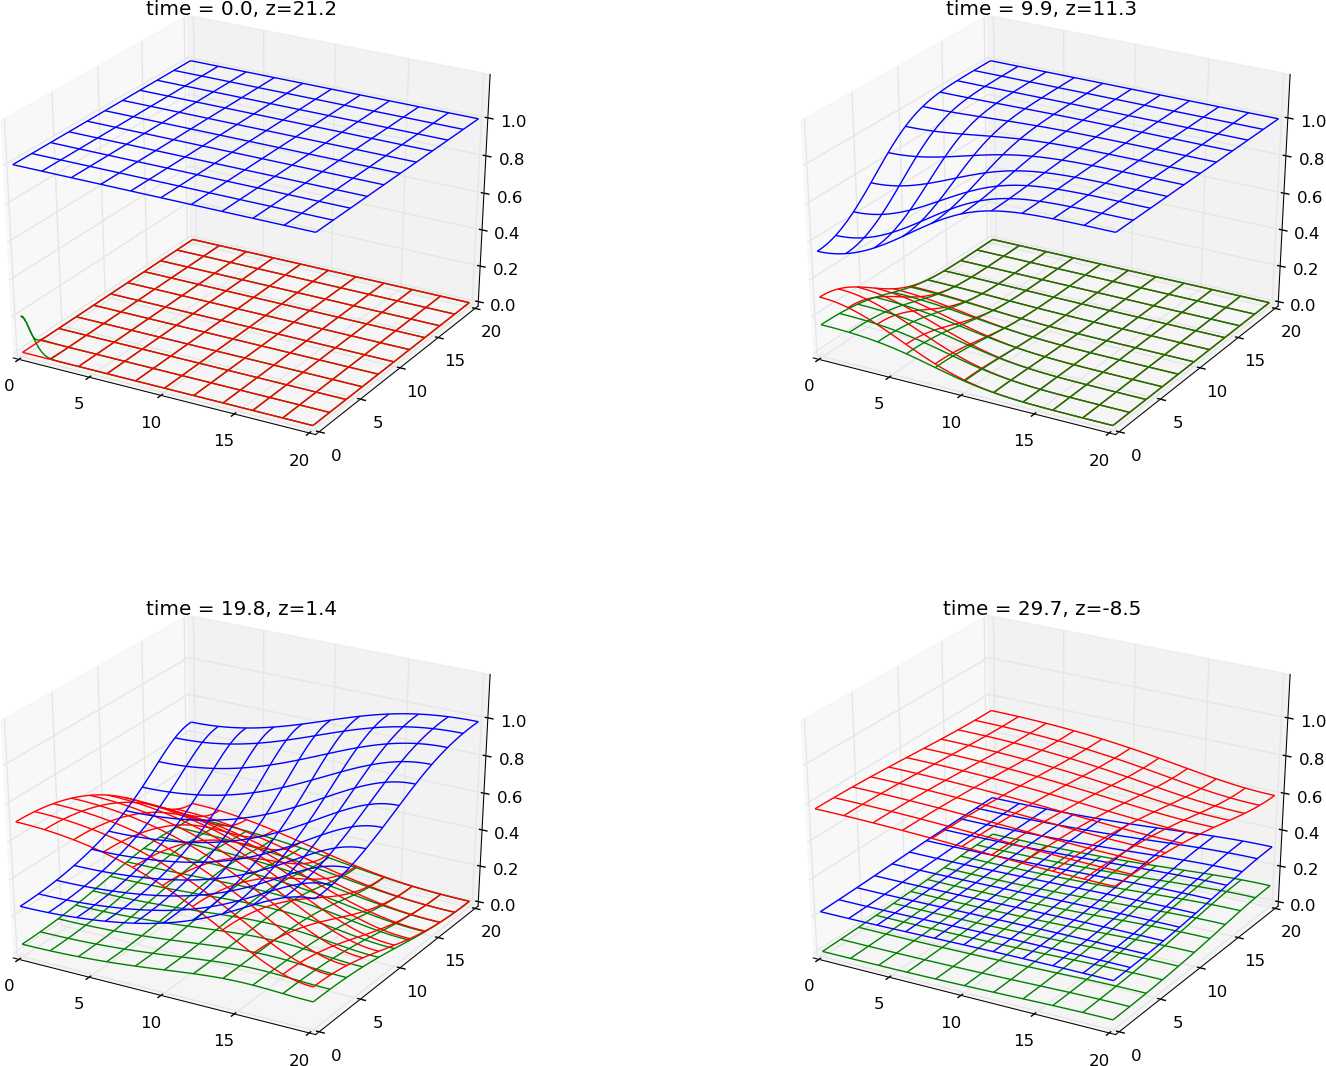
\includegraphics[width=0.8\linewidth]{plots/2D_gauss_one_sub.eps}}
  \caption{
  A gaussian function from $x=0,y=0$ based on the PDE system (\ref{eq:simple_non_PDE}) with $\lambda=0.5$
  }
\end{figure}
%\clearpage % flush figures 


\subsection{2D Gaussian function from x=0,y=0 with higher initial value}

\subsection{English Boarding School}


\begin{center}  % inline figure
  \centerline{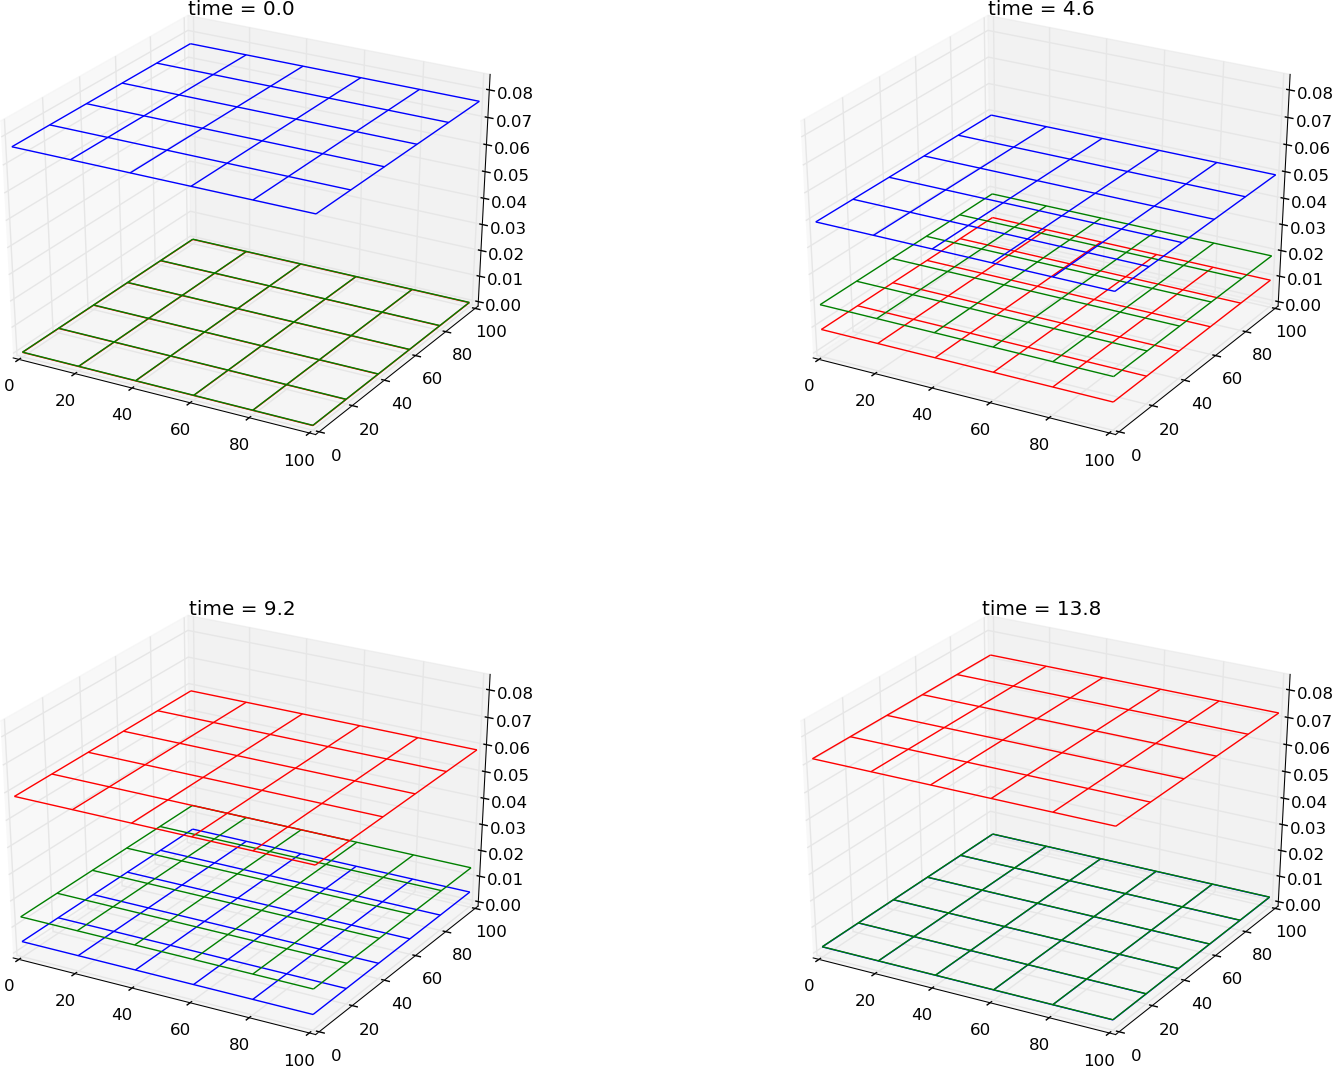
\includegraphics[width=0.8\linewidth]{plots/2D_british_school_sub.eps}}
\end{center}


\paragraph{Gaussian from the corner.}
\begin{center}  % inline figure
  \centerline{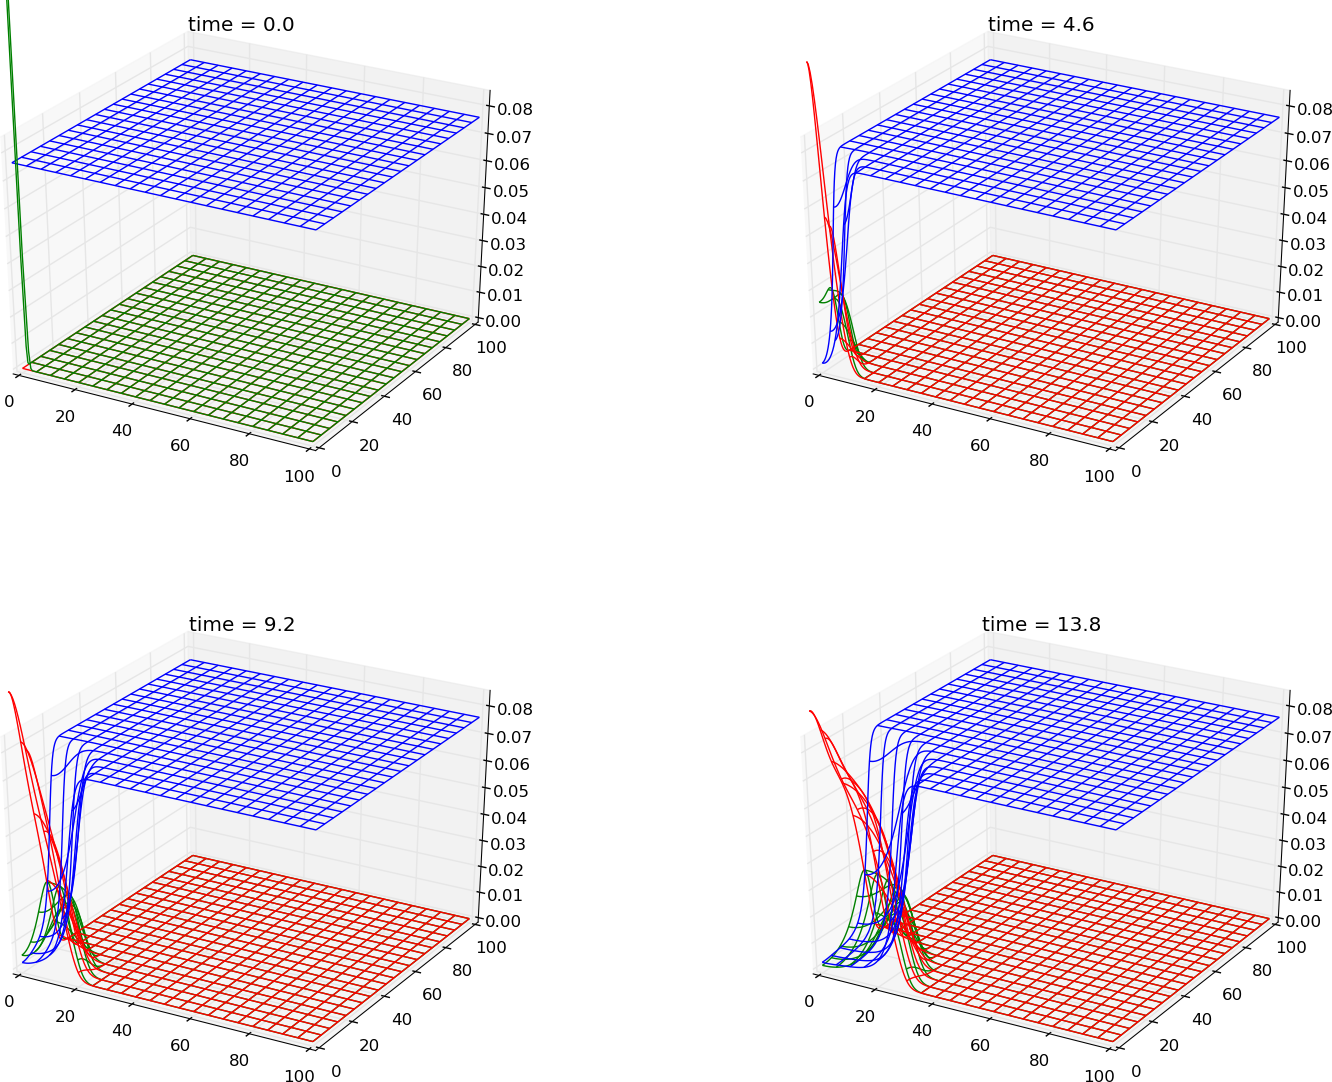
\includegraphics[width=0.8\linewidth]{plots/2D_british_school_gauss_corner_sub.eps}}
\end{center}


\paragraph{A long simulation on 100 Days.}
\begin{center}  % inline figure
  \centerline{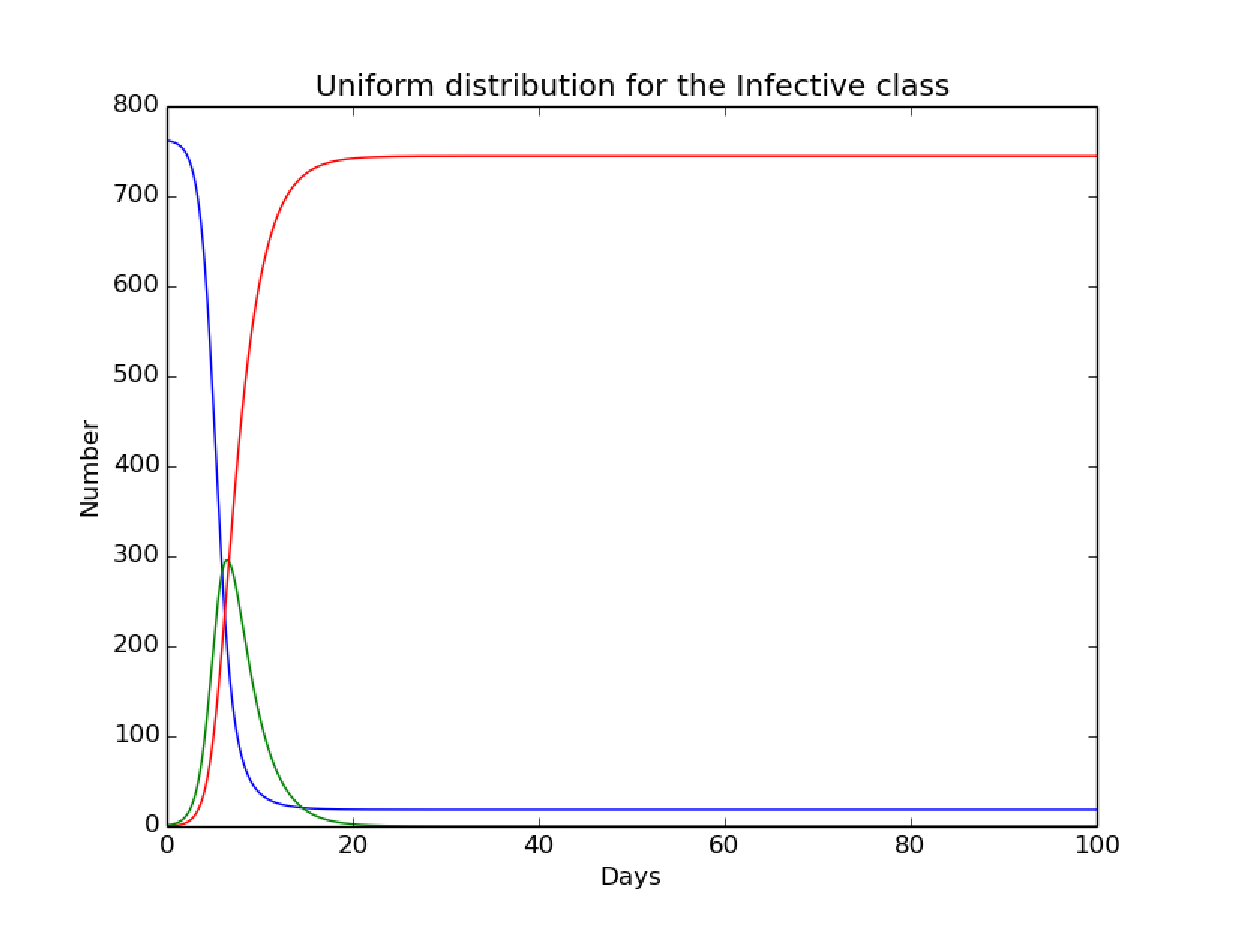
\includegraphics[width=0.8\linewidth]{plots/2D_british_school_long_number.eps}}
\end{center}



\begin{center}  % inline figure
  \centerline{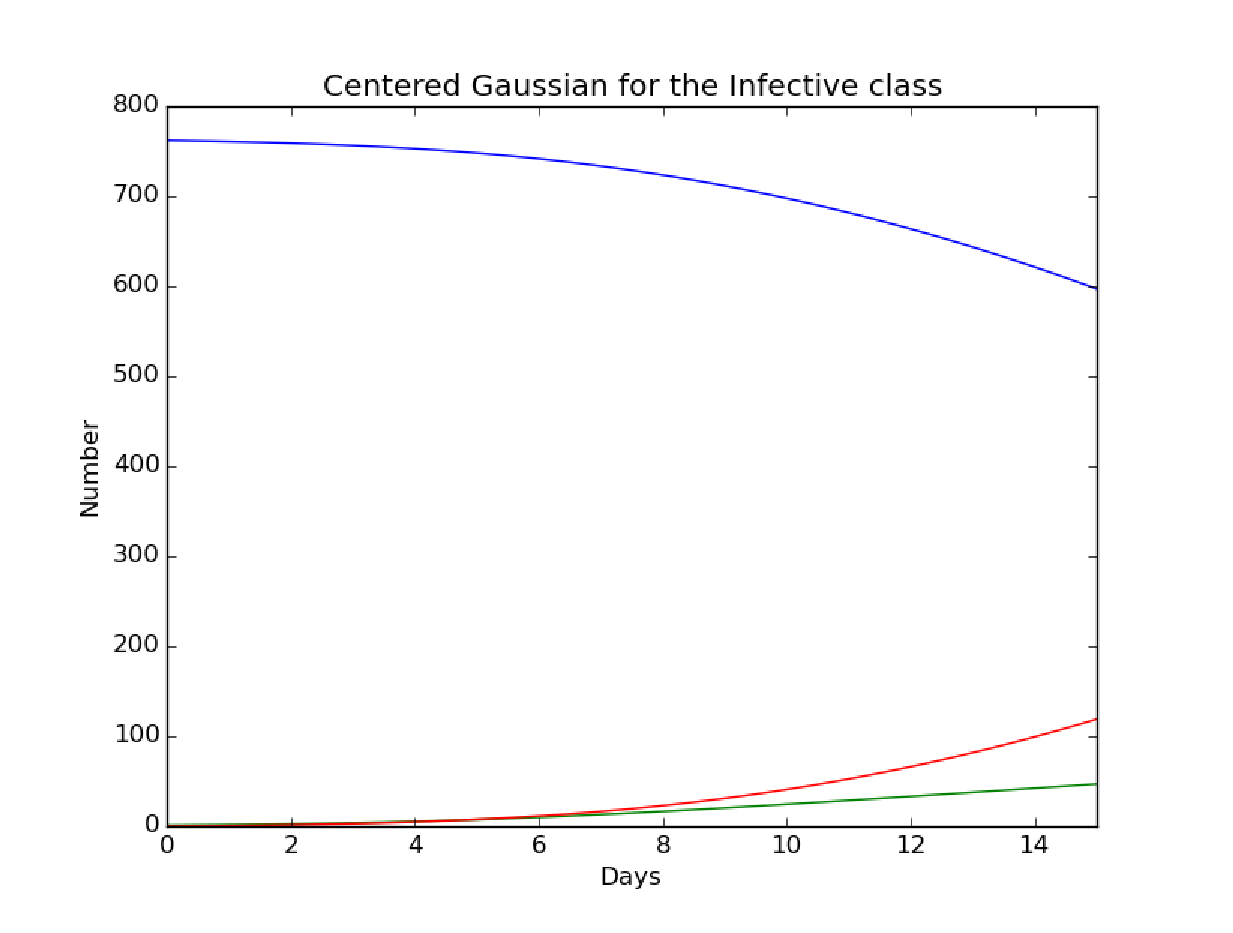
\includegraphics[width=0.8\linewidth]{plots/2D_british_school_gauss_long_number.eps}}
\end{center}



\begin{center}  % inline figure
  \centerline{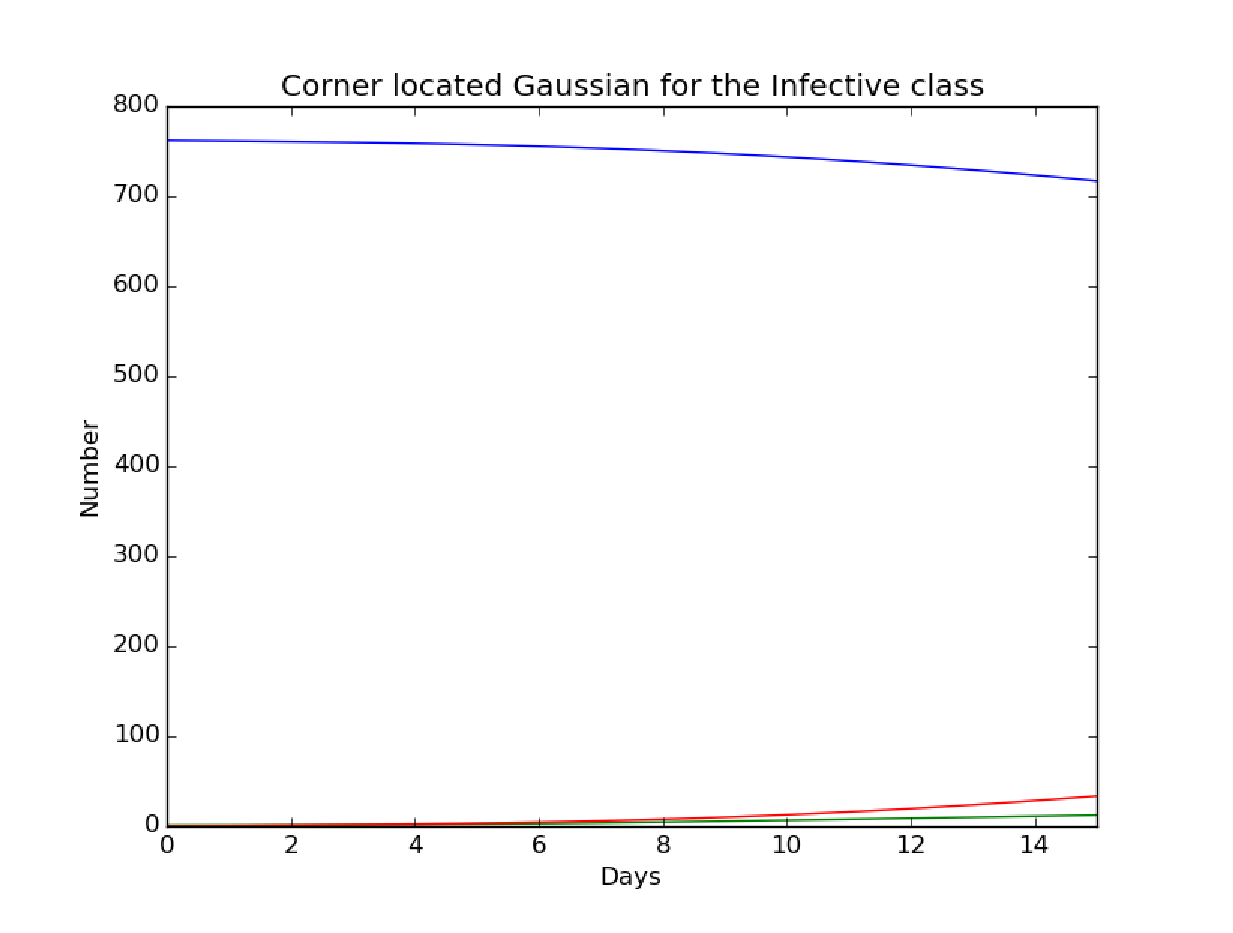
\includegraphics[width=0.8\linewidth]{plots/2D_british_school_gauss_corner_long_number.eps}}
\end{center}


\subsection{Zombiefication}
\paragraph{Verify the initial phase.}
\begin{center}  % inline figure
  \centerline{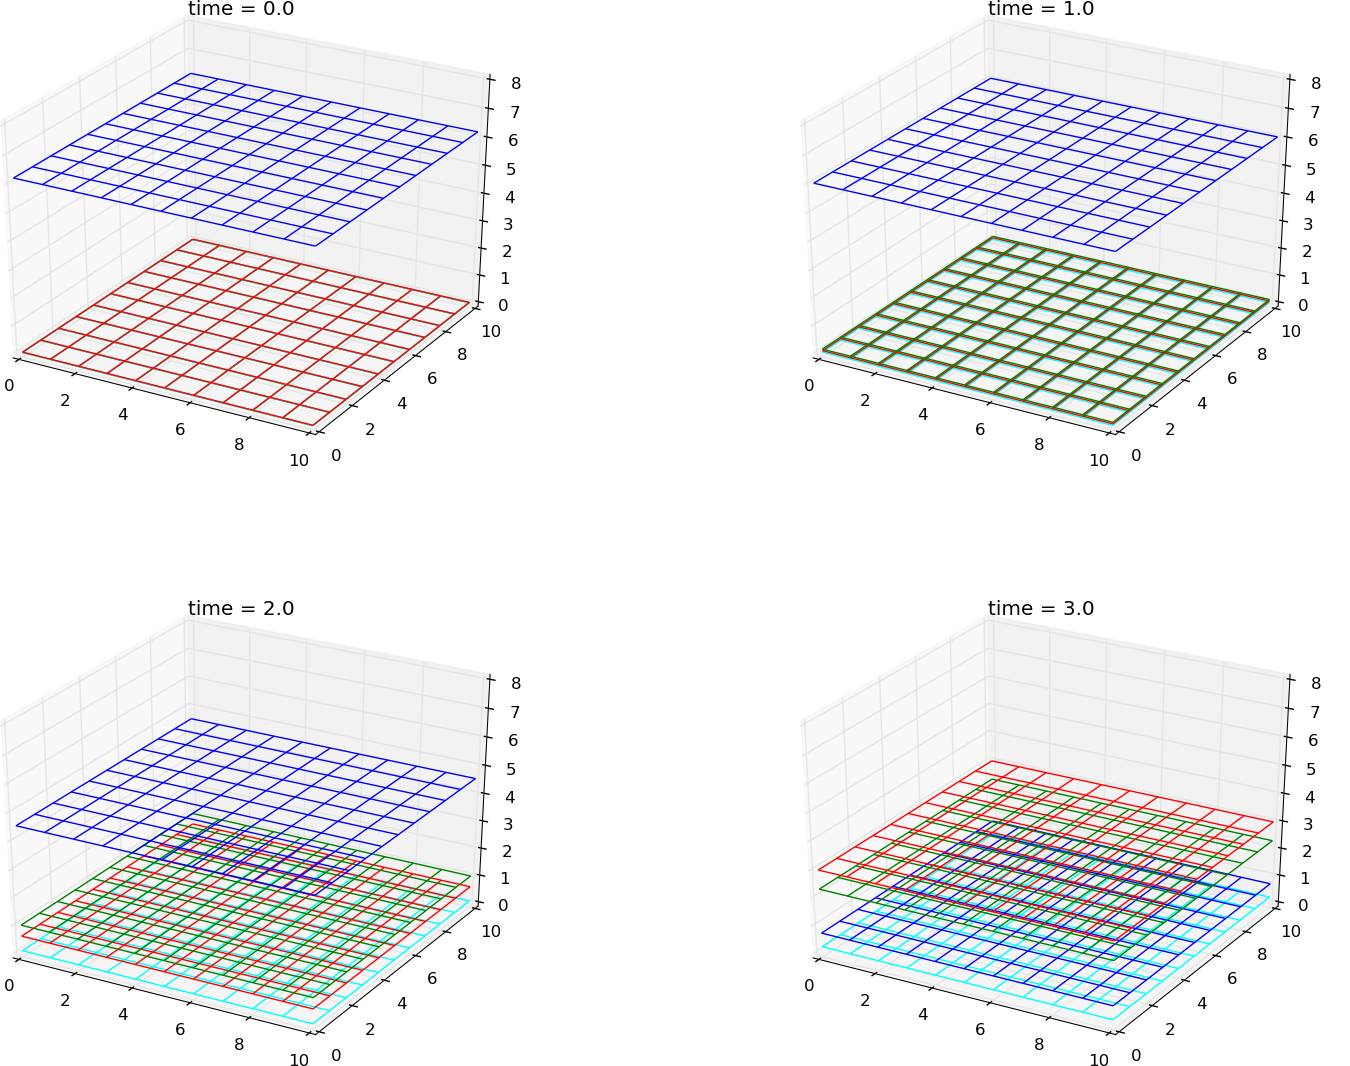
\includegraphics[width=0.8\linewidth]{plots/2D_zombie_initial_cond_sub.eps}}
\end{center}



\begin{figure}[ht]
  \centerline{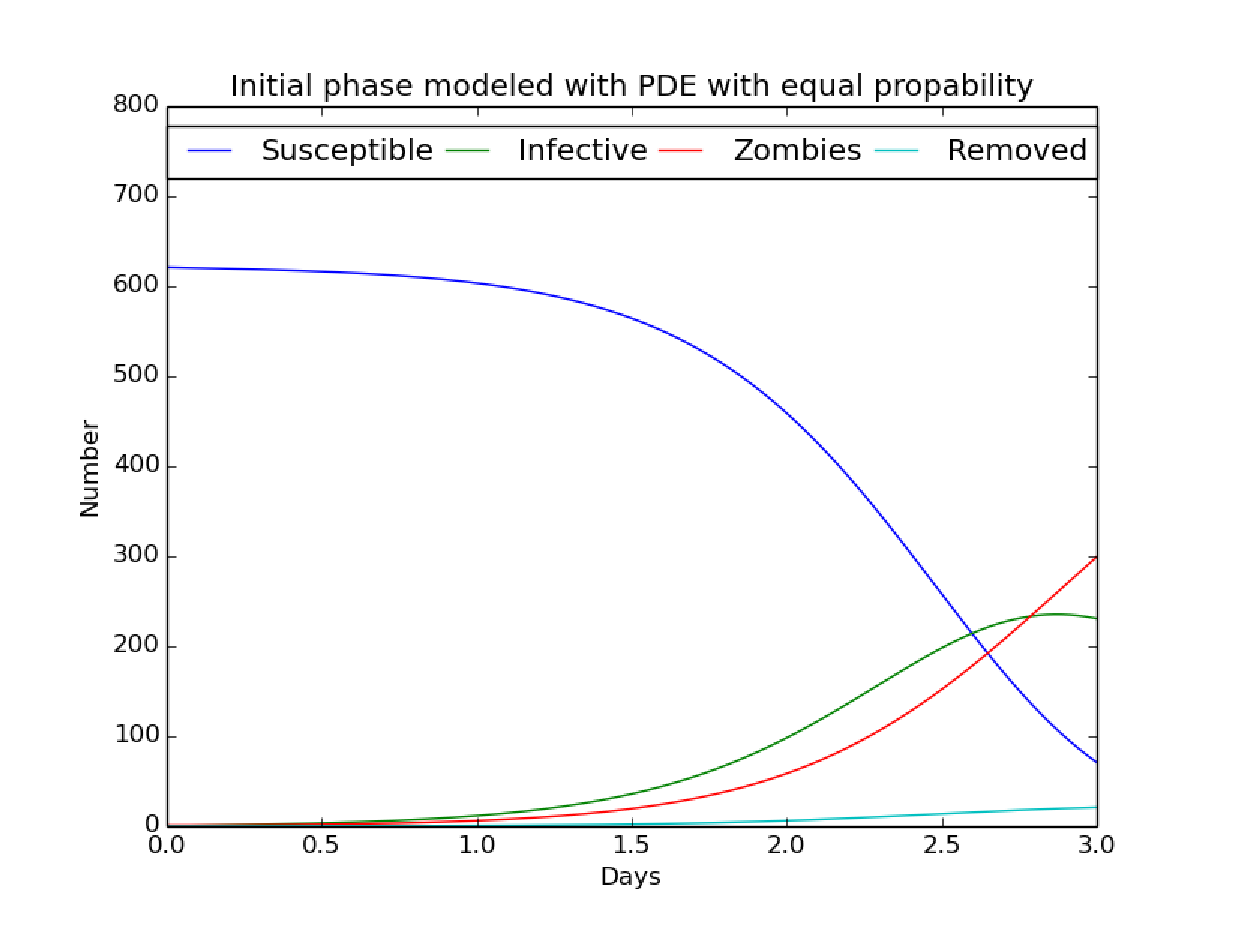
\includegraphics[width=0.8\linewidth]{plots/2D_zombie_initial_cond_number.eps}}
  \caption{
  Creates the same results as for the ODE system
  }
\end{figure}
%\clearpage % flush figures 


\paragraph{Three phases.}
\begin{center}  % inline figure
  \centerline{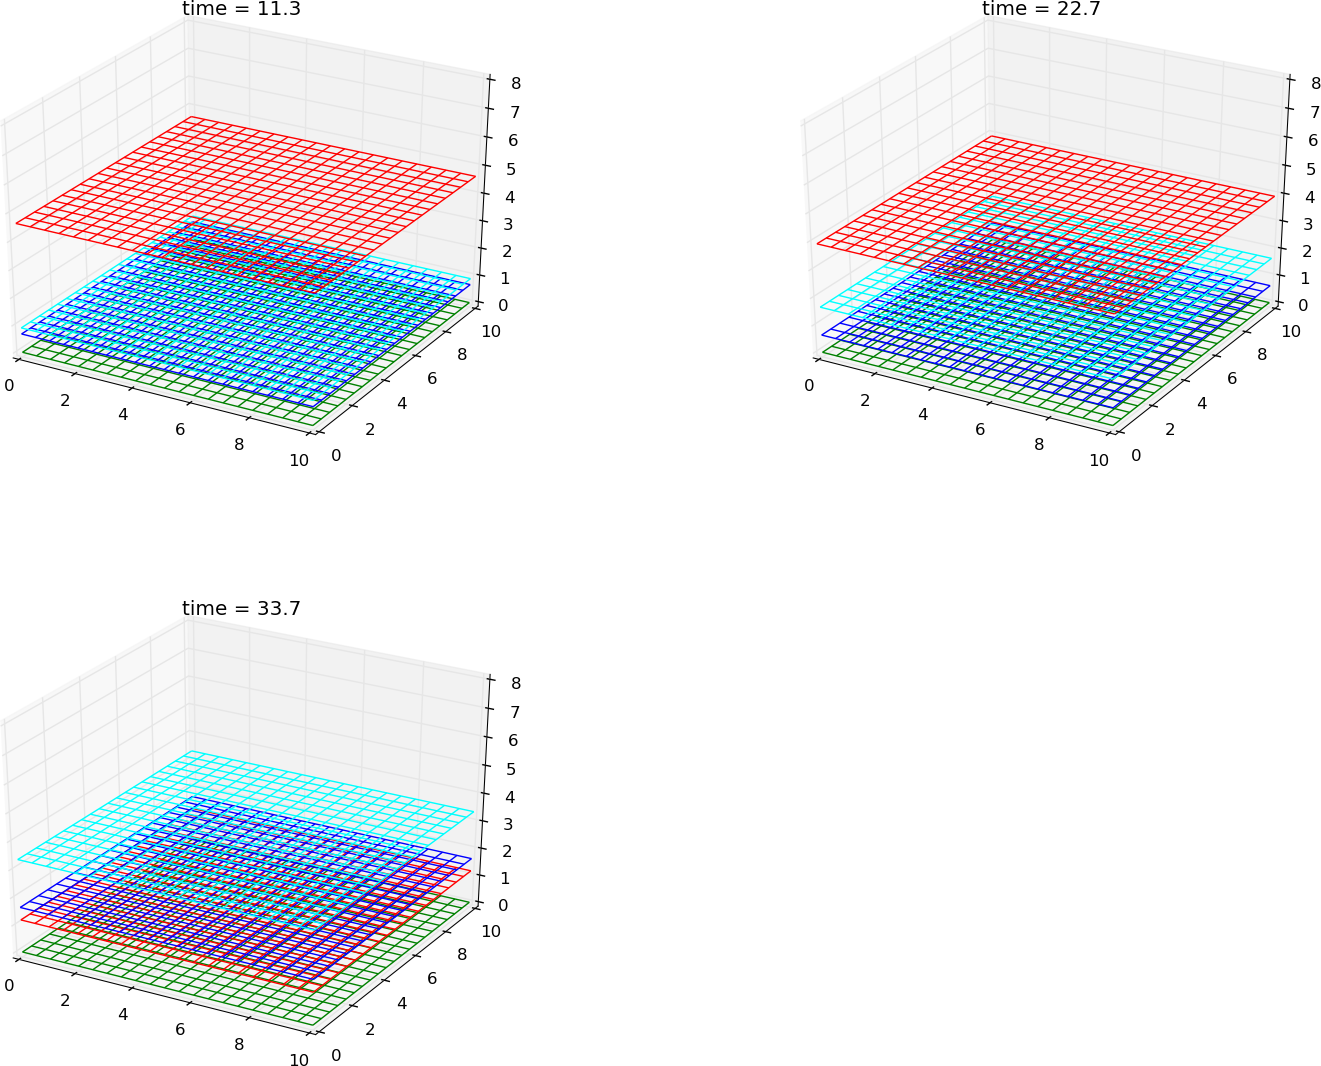
\includegraphics[width=0.8\linewidth]{plots/2D_zombie_three_phases_sub.eps}}
\end{center}


\paragraph{middle town.}
\begin{center}  % inline figure
  \centerline{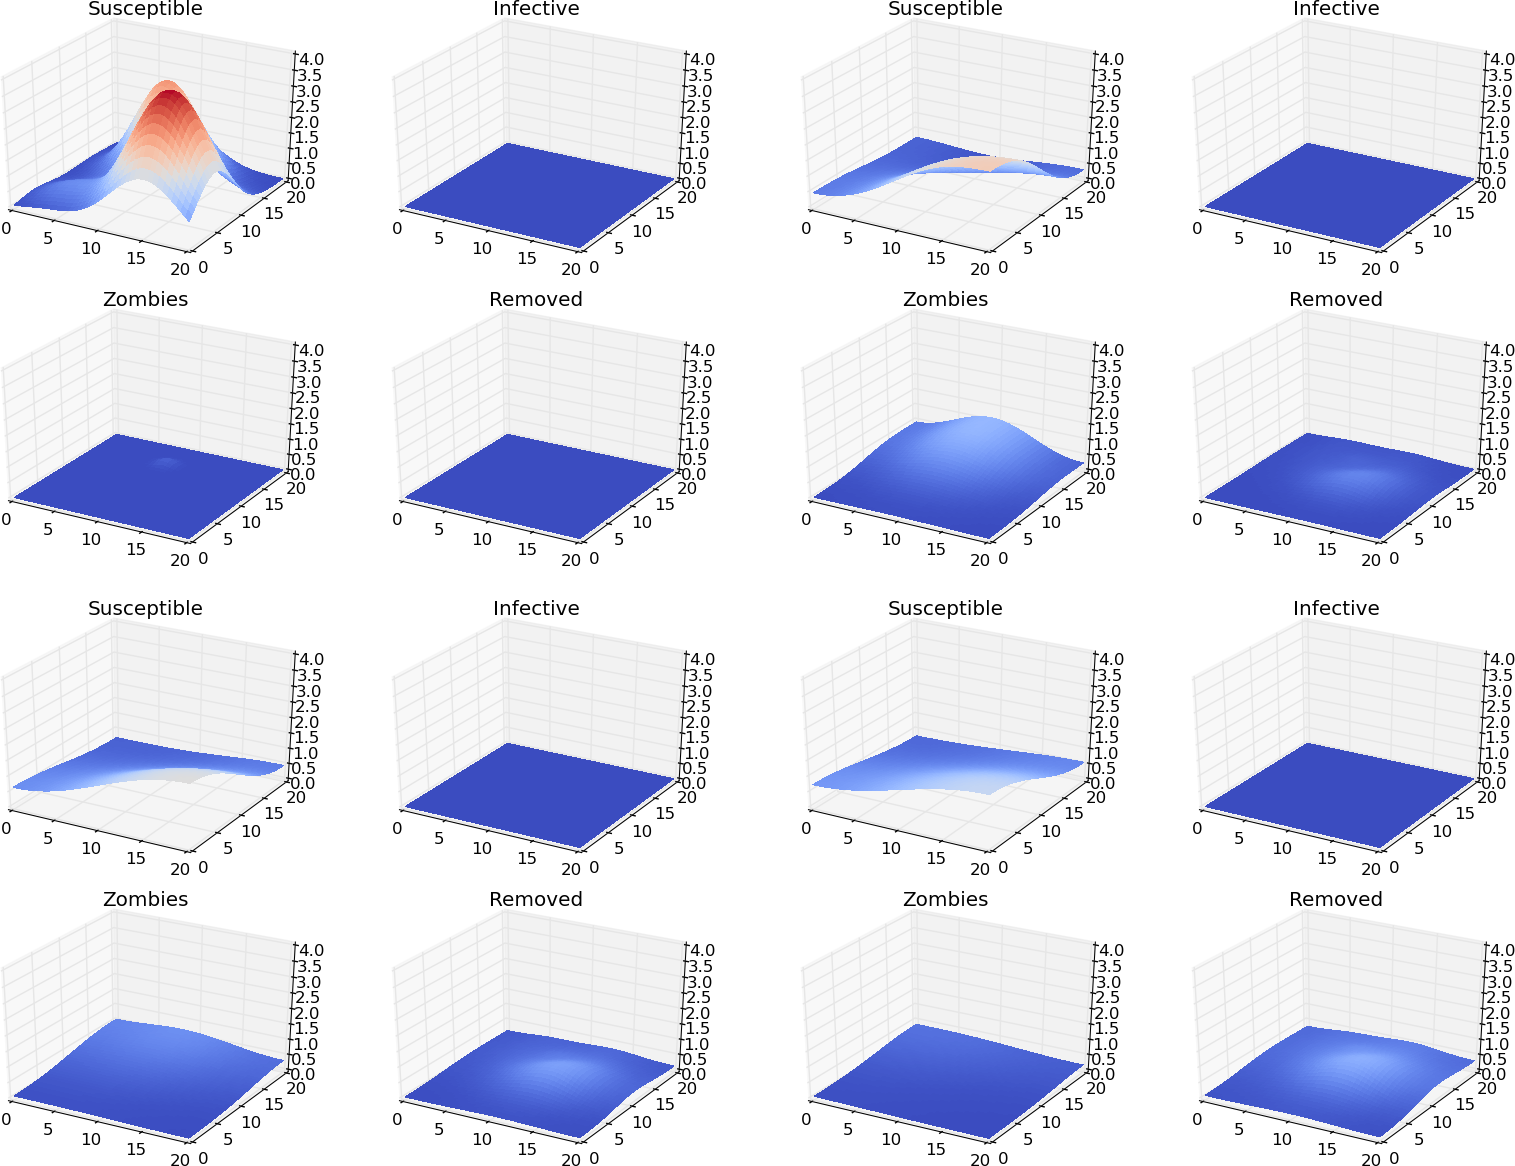
\includegraphics[width=0.8\linewidth]{plots/2D_zombie_three_phases_zombie_middle_town_surface_sub.eps}}
\end{center}


\paragraph{large town.}
\begin{center}  % inline figure
  \centerline{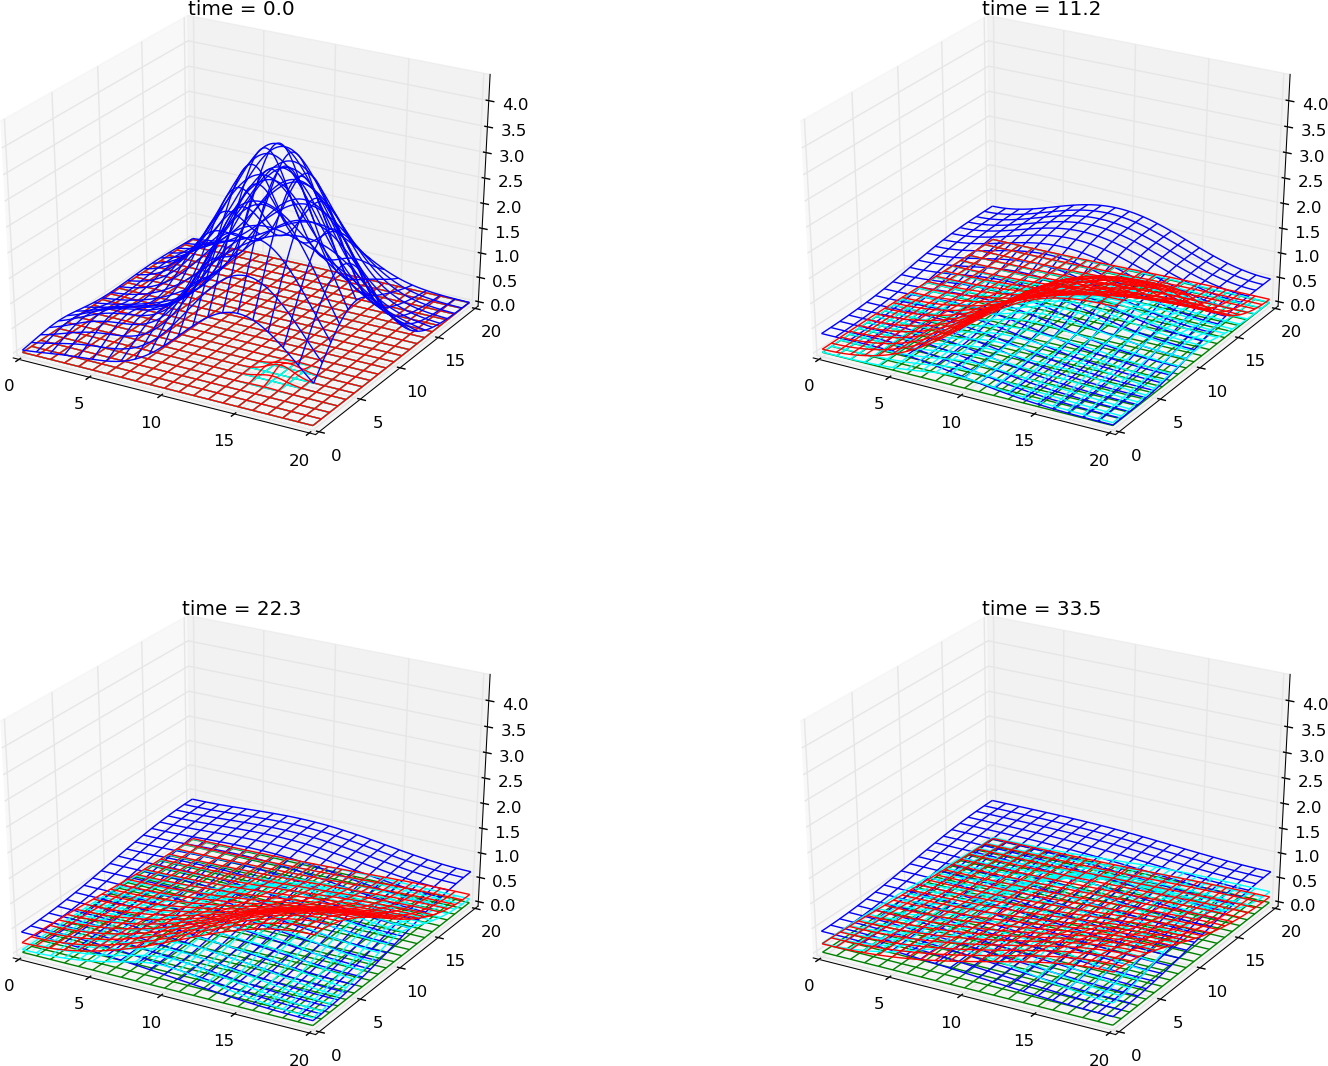
\includegraphics[width=0.8\linewidth]{plots/2D_zombie_three_phases_zombie_large_town_sub.eps}}
\end{center}


% MOVIE:[plots/2D_gaussian.webm, height=500 width=600] Travelling wave modeled with the same values as for 1D.
% MOVIE:[plots/2D_one_corner.webm, height=500 width=600] Starting the travelling wave from the corner.
% MOVIE:[plots/2D_initial_variable.webm, height=500 width=600] Travelling wave with a greater initial wave.
% MOVIE:[plots/2D_british_school.webm, height=500 width=600] Acts like the ODE system
% MOVIE:[plots/2D_british_school_gauss.webm, height=500 width=600] The sick one is placed in the center of the School area.
% MOVIE:[plots/2D_british_school_gauss_corner.webm, height=500 width=600] A wave of infected moves towards the school yard
% MOVIE:[plots/2D_zombie_initial_cond.webm, height=500 width=600]
% MOVIE:[plots/2D_zombie_three_phases.webm, height=500 width=600]
% MOVIE:[plots/2D_zombie_three_phases_zombie_small_town.webm, height=500 width=600] Created with different diffusion constants. The groups of susceptible are placed in three different areas.
% MOVIE:[plots/2D_zombie_three_phases_zombie_small_town_surface.webm, height=500 width=600] Created with different diffusion constants. The groups of susceptible are placed in three different areas.
% MOVIE:[plots/2D_zombie_three_phases_zombie_middle_town.webm, height=500 width=600] Created with different diffusion constants. The groups of susceptible are placed in three different areas.
% MOVIE:[plots/2D_zombie_three_phases_zombie_middle_town_surface.webm, height=500 width=600] Created with different diffusion constants. The groups of susceptible are placed in three different areas.
% MOVIE:[plots/2D_zombie_three_phases_zombie_large_town.webm, height=500 width=600] Created with different diffusion constants. The groups of susceptible are placed in three different areas.
% MOVIE:[plots/2D_zombie_three_phases_zombie_large_town_surface.webm, height=500 width=600] Created with different diffusion constants. The groups of susceptible are placed in three different areas.
% MOVIE:[plots/2D_zombie_three_phases_blindern_area_contourf.webm, height=500 width=600] Created with different diffusion constants. The groups of susceptible are placed in three different areas.
% MOVIE:[plots/2D_zombie_three_phases_blindern_area_3_ph_contourf.webm, height=500 width=600] Created with different diffusion constants. The groups of susceptible are placed in three different areas.




\bibliographystyle{plain}
\bibliography{../bibliography/papers}


% ------------------- end of main content ---------------


% #ifdef PREAMBLE
\printindex

\end{document}
% #endif

